%! TeX program = lualatex
\documentclass[10pt, aspectratio=169]{beamer}

% Draft
\newif\ifisdraft
\isdraftfalse

\usepackage{beamer-reveal}
\usetheme[]{metropolis}

\AtBeginSection{
  \frame[plain,c,noframenumbering]{
    \sectionpage
    \begin{center}
      % \begin{multicols}{2}  % 2 columns, auto-balances
      %   \raggedcolumns
      %   \raggedright
      %   \tableofcontents[currentsection, hideothersubsections]
      % \end{multicols}
     \begin{columns}[t]
        \begin{column}{.5\textwidth}
            \tableofcontents[sections={1-3}, currentsection, hideothersubsections]
        \end{column}
        \begin{column}{.5\textwidth}
            \tableofcontents[sections={4-6}, currentsection, hideothersubsections]
        \end{column}
    \end{columns}
    \end{center}
  }
}

\setbeamerfont{page number in head/foot}{size=\tiny}
\setbeamercolor{footline}{fg=gray!70}

% Footline highlight
\colorlet{footlineHlColor}{black!60}
\newcommand{\footlineHl}[1]{
  \textbf{\textcolor{footlineHlColor}{#1}}
}

\setbeamercolor{title page}{bg=white, fg=black}
\defbeamertemplate*{title page}{customized}[1][]
{
  \centering

  % --- Main title box ---
  \begin{beamercolorbox}[
    wd=\textwidth,
    sep=1.2em,
    rounded=true
  ]{title page}
    
    {\usebeamerfont{title}\inserttitle\par}
    \vspace{0.4em}

    {\usebeamerfont{subtitle}\usebeamercolor[fg]{subtitle}\insertsubtitle\par}

    \vspace{0.8em}

    {\usebeamerfont{author}\insertauthor\par}
    {\usebeamerfont{institute}\insertinstitute\par}
    {\usebeamerfont{date}\insertdate\par}

  \end{beamercolorbox}

  \vfill

  % --- Logos (outside the box) ---
  \usebeamercolor[fg]{titlegraphic}\inserttitlegraphic
}

\defbeamertemplate*{footline}{customized}{%
  \leavevmode%
  \hbox{%
    \begin{beamercolorbox}[wd=.1\textwidth,left,sep=1.5ex]{footline}%
    \end{beamercolorbox}%
    \begin{beamercolorbox}[wd=.8\textwidth,center,sep=1.5ex]{footline}%
      \usebeamertemplate*{frame footer}%
    \end{beamercolorbox}%
    \begin{beamercolorbox}[wd=.1\textwidth,right,sep=1.5ex]{footline}%
      \usebeamerfont{page number in head/foot}%
      \hfill%
      \usebeamertemplate*{frame numbering}
    \end{beamercolorbox}%
  }%
}
\makeatletter
  \setbeamertemplate{frametitle}{%
    \begin{beamercolorbox}[%
      wd=1.0\paperwidth,%
      sep=0pt,%
      leftskip=\metropolis@frametitle@padding,%
      rightskip=\metropolis@frametitle@padding,%
      ]{frametitle}%
      \metropolis@frametitlestrut@start%
      \insertframetitle%
      \ifx\insertframesubtitle\@empty%
      \else%
        \hfill%
        {\usebeamerfont{framesubtitle}\usebeamercolor[fg]{framesubtitle}\insertframesubtitle}%
      \fi%
      \nolinebreak%
      \metropolis@frametitlestrut@end%
    \end{beamercolorbox}%
  }
\makeatother



\usepackage{caption}
\captionsetup{font=scriptsize,labelfont=scriptsize}
\usepackage{subcaption}
\usepackage{siunitx}
\sisetup{
  range-phrase = --,
  range-units = single,
}
\usepackage{multirow}
\usepackage{booktabs}

\usepackage{cleveref}

\usepackage{natbib}

\usepackage{pifont}
\usepackage{wasysym}

\usepackage{bm}

% PSEUDO-CODE
\usepackage{algorithm}
\usepackage[
  rightComments=false,
]{algpseudocodex}
\colorlet{commentcolor}{gray!25}

\usepackage{stackengine}
\usepackage{changepage}

% CASTEL PACKAGES
\usepackage{import}
\usepackage{xifthen}
\usepackage{transparent}
% END CASTEL PACKAGES
\newcommand{\castelincfig}[2][1.0]{%
  \def\svgwidth{#1\columnwidth} \import{./figures/}{#2.pdf_tex}
}

% Math commands
\newcommand{\dependson}[1]{
  {\scriptstyle(#1)}
}

\usepackage{tikz}
\usetikzlibrary{external}
% \tikzexternalize[prefix=tikz-cache/]

\usepackage{calc}
\usepackage{pgfplots}\pgfplotsset{compat=newest}
\usetikzlibrary{decorations.pathreplacing,calc,positioning,spy,pgfplots.units,chains,backgrounds}
\usepgfplotslibrary{groupplots}
\tikzset{
  annotate box/.style={
    fill=white,
    fill opacity=.4,
    text opacity=1,
    rounded corners=2pt,
    inner xsep=4pt,
    inner ysep=3pt,
    draw=black,
    line width=.4pt,
  },
}
\usepackage[most]{tcolorbox}

\title{Computational strategies for time-accurate simulation of part-scale LPBF}
\subtitle{Time scale disparity in moving heat source problems}
\author[Mehdi Slimani]{
Mehdi Slimani \qquad \qquad
{\footnotesize
  \begin{tabular}{rl}
    Supervised by & Prof. Michele Chiumenti \\
                  & Prof. Miguel Cervera
  \end{tabular}
}}
\date{January 23, 2026}
\titlegraphic{%
  \vfill
  {
  \centering
  \begin{minipage}[t]{0.3\textwidth}
    \vfill
    \includegraphics[height=0.1\pageheight]{logos/UPC_Camins.png}
  \end{minipage}%
  \begin{minipage}[t]{0.3\textwidth}
    \centering
    \footnotesize
    Doctoral Degree in Structural Analysis\\[0.5cm]
    Thesis submitted as a compendium of publications
  \end{minipage}%
  \begin{minipage}[t]{0.3\textwidth}
    \vfill
    \hfill
    \includegraphics[height=0.1\pageheight]{logos/CIMNE-black.png}%
  \end{minipage}
  }
}

\graphicspath{{figures/}}

\newif\ifisdraft
\isdraftfalse
\newcommand{\isdraft}{\ifisdraft true\else false\fi}
\newcommand{\todo}[1]{
  \ifisdraft {
    \Large
    $\color{black}\star$\color{red}~\textit{#1}\color{black}~$\star$
  } \fi
}

% Used in advected_subdomain.tex
\definecolor{advectionColor}{RGB}{213,94,0}   % vermillion / orange
\definecolor{diffusionColor}{RGB}{0,114,178}  % blue

\definecolor{powderColor}{rgb}{0.878,0.859,0.811}
\definecolor{metalColor}{rgb}{0.420,0.408,0.384}
\newcommand{\legendpowderbulk}{%
  \begin{tabular}{rlrl}
     ({\color{powderColor} \rule[-1.5 pt]{8 pt}{8 pt}}) & Powder & ({\color{metalColor} \rule[-1.5 pt]{8 pt}{8 pt}})  & Bulk
  \end{tabular}
}
\newcommand{\wireframeTriangle}{%
    \begin{tikzpicture}[scale=0.2] % adjust scale as needed
      % Bottom triangle
      \draw[]
        (0,0) coordinate (A)
        -- (0,1) coordinate (B)
        -- (1,0) coordinate (C)
        -- cycle;
      % Upper triangle
      \draw[]
        (0,1) coordinate (D)
        -- (1,1) coordinate (E)
        -- (1,0) coordinate (F);
    \end{tikzpicture}
}

\newcommand{\playthumb}[2][]{%
  \begin{tikzpicture}
    % Thumbnail image
    \node[inner sep=0] (img) {\includegraphics[#1]{#2}};
    % Dark circle
    \draw[fill=black!60, draw=white, line width=0.8pt]
      (img.center) circle[radius=0.6cm];
    % Triangle
    \draw[fill=white, draw=none, rounded corners=1.5pt]
      ([xshift=0.34cm]img.center) --
      ([xshift=-0.19cm,yshift=0.3cm]img.center) --
      ([xshift=-0.19cm,yshift=-0.3cm]img.center) -- cycle;
  \end{tikzpicture}%
}

\newcounter{video}
\renewcommand{\thevideo}{Video \arabic{video}}
\newcommand{\videoCaption}[1]{%
  \captionof{video}{#1}%
}

\newcommand{\externalvod}[3]{\movie[externalviewer]{\playthumb[#1]{#3}}{#2}}
\newcommand{\seudoembeddedvod}[3]{\movie[poster, showcontrols]{\playthumb[#1]{#3}}{#2}}

\DeclareRobustCommand{\labelbox}[2][]{%
  % Inline TikZ node; safe in text, math, tabular, makebox, etc.
  \tikz[baseline=(X.base)]\node[annotate box,#1] (X) {#2};%
}
\newcommand{\support}[1]{\text{supp}\left(#1\right)}
\newcommand{\nablaxi}[0]{\nabla_{\boldsymbol{\xi}}}
\newcommand{\deltaxi}[0]{\Delta_{\boldsymbol{\xi}}}
\newcommand{\eunorm}[1]{
  \text{\Large$|\hspace{-0.8mm}|$}\; #1 \;\text{\Large$|\hspace{-0.8mm}|_{\scriptscriptstyle{2}}$}
}

\pgfplotsset{
  colormap={rainbow}{
    rgb255(0.0cm)=(5,97,254);
    rgb255(0.023809523809523808cm)=(5,108,247);
    rgb255(0.047619047619047616cm)=(5,119,239);
    rgb255(0.07142857142857142cm)=(5,130,232);
    rgb255(0.09523809523809523cm)=(5,139,222);
    rgb255(0.11904761904761904cm)=(5,148,212);
    rgb255(0.14285714285714285cm)=(5,157,202);
    rgb255(0.16666666666666666cm)=(5,166,191);
    rgb255(0.19047619047619047cm)=(5,174,179);
    rgb255(0.21428571428571427cm)=(5,183,167);
    rgb255(0.23809523809523808cm)=(5,193,153);
    rgb255(0.2619047619047619cm)=(5,202,140);
    rgb255(0.2857142857142857cm)=(5,211,126);
    rgb255(0.30952380952380953cm)=(5,220,109);
    rgb255(0.3333333333333333cm)=(5,228,91);
    rgb255(0.35714285714285715cm)=(4,237,74);
    rgb255(0.38095238095238093cm)=(69,242,39);
    rgb255(0.40476190476190477cm)=(125,245,28);
    rgb255(0.42857142857142855cm)=(164,249,11);
    rgb255(0.4523809523809524cm)=(194,251,8);
    rgb255(0.47619047619047616cm)=(224,252,5);
    rgb255(0.5cm)=(254,254,3);
    rgb255(0.5238095238095238cm)=(254,243,20);
    rgb255(0.5476190476190477cm)=(254,232,37);
    rgb255(0.5714285714285714cm)=(254,220,55);
    rgb255(0.5952380952380952cm)=(254,208,55);
    rgb255(0.6190476190476191cm)=(254,196,55);
    rgb255(0.6428571428571429cm)=(254,183,55);
    rgb255(0.6666666666666666cm)=(254,171,55);
    rgb255(0.6904761904761905cm)=(254,159,55);
    rgb255(0.7142857142857143cm)=(254,147,55);
    rgb255(0.7380952380952381cm)=(254,132,55);
    rgb255(0.7619047619047619cm)=(254,118,55);
    rgb255(0.7857142857142857cm)=(254,104,55);
    rgb255(0.8095238095238095cm)=(253,84,53);
    rgb255(0.8333333333333334cm)=(251,66,48);
    rgb255(0.8571428571428571cm)=(252,37,53);
    rgb255(0.8809523809523809cm)=(242,29,64);
    rgb255(0.9047619047619048cm)=(230,20,74);
    rgb255(0.9285714285714286cm)=(218,10,84);
    rgb255(0.9523809523809523cm)=(203,11,91);
    rgb255(0.9761904761904762cm)=(189,11,98);
    rgb255(1.0cm)=(174,12,105);
  }
}
\pgfplotsset{
  colormap={fast}{
    rgb255(0.0cm)=(22,47,140);
    rgb255(0.16144cm)=(56,131,180);
    rgb255(0.351671cm)=(128,220,221);
    rgb255(0.501285cm)=(255,255,211);
    rgb255(0.620051cm)=(240,227,138);
    rgb255(0.835408342528245cm)=(191,113,65);
    rgb255(1.0cm)=(142,14,14);
  }
}
\pgfplotsset{
  colormap={rainbow_blended_white}{
    rgb(0cm)=(1, 1, 1);
    rgb(0.17cm)=(0, 0, 1);
    rgb(0.34cm)=(0, 1, 1);
    rgb(0.5cm)=(0, 1, 0);
    rgb(0.67cm)=(1, 1, 0);
    rgb(0.84cm)=(1, 0, 0);
    rgb(1cm)=(0.878431372549, 0, 1);
  }
}
\pgfplotsset{
  colormap={powderbulk}{
    rgb255(0cm)=(224,219,207);
    rgb255(0.499cm)=(224,219,207);
    rgb255(0.501cm)=(107.0,104.0,98.0);
    rgb255(1cm)=(107.0,104.0,98.0);
  }
}

\newcommand{\vcolorbar}[6]{
  \begin{tikzpicture}
    \pgfmathsetmacro{\myheight}{10*#2}
    \pgfmathsetmacro{\widthcolorbar}{#2}
    \pgfmathsetmacro{\cmin}{#3}
    \pgfmathsetmacro{\cmax}{#4}
    \def\extraticks{#6}
    \ifx\extraticks\empty
      \def\ticklist{0,1}
    \else
      \def\ticklist{0,\extraticks,1}
    \fi
    \begin{axis}[
      hide axis,
      scale only axis,
      height=\myheight,
      width=\widthcolorbar,
      colormap name={#1},
      colorbar,
      colorbar style={
        ytick={\ticklist},
        yticklabel pos=right,
        yticklabel style={font=\footnotesize},
        yticklabel={
          \pgfmathparse{\cmin+(\cmax-\cmin)*\tick}\pgfmathprintnumber[precision=1, fixed]{\pgfmathresult}
        },
        ylabel=#5,
        ylabel style={
          at={(0.0,0.5)},
          anchor=south,
          rotate=0,
          font=\footnotesize,
          overlay,
        },
        yticklabel style={
          font=\footnotesize,
          overlay,
        },
        width=\widthcolorbar,
      },
      point meta min=0,
      point meta max=1,
    ]
      % dummy plot just to draw colorbar:
      \addplot [draw=none] coordinates {(0,0) (0,1)};
    \end{axis}
  \end{tikzpicture}
}
\newcommand{\hcolorbar}[6]{
  \begin{tikzpicture}
    \pgfmathsetmacro{\myheight}{#2}
    \pgfmathsetmacro{\widthcolorbar}{10*#2}
    \pgfmathsetmacro{\cmin}{#3}
    \pgfmathsetmacro{\cmax}{#4}
    \def\extraticks{#6}
    \ifx\extraticks\empty
      \def\ticklist{0,1}
    \else
      \def\ticklist{0,\extraticks,1}
    \fi
    \begin{axis}[
      hide axis,
      scale only axis,
      height=\myheight,
      width=\widthcolorbar,
      colormap name={#1},
      colorbar horizontal,
      colorbar style={
        xtick={\ticklist},
        xticklabel pos=left,
        xticklabel style={font=\footnotesize},
        xticklabel={
          \pgfmathparse{\cmin+(\cmax-\cmin)*\tick}\pgfmathprintnumber[precision=1, fixed]{\pgfmathresult}
        },
        xticklabel style={font=\footnotesize},
        xlabel=#5,
        xlabel style={at={(0.5,1.0)}, rotate=0, anchor=south, font=\footnotesize},,
        width=\widthcolorbar,
      },
      point meta min=0,
      point meta max=1,
    ]
      % dummy plot just to draw colorbar:
      \addplot [draw=none] coordinates {(0,0) (0,1)};
    \end{axis}
  \end{tikzpicture}
}


\pgfplotsset{
  convplotstyle/.style={
    clip=true,
    xlabel={$\Delta t_{f} [T_{hs}]$},
    ylabel={$||u_h - u_{ex}||_2$},
    grid=major,
    xtick={1,0.5,0.25,0.125,0.0625},
    xticklabels={$1$,$\tfrac{1}{2}$,$\tfrac{1}{4}$,$\tfrac{1}{8}$,$\tfrac{1}{16}$},
    x dir=reverse,
    scale only axis,
  },
  oscillationstyle/.style={
    clip=true,
    enlargelimits=false,
    ymin=25.0,
    ymax=2400.0,
    grid=major,
    ytick={25,400,900,1300,1625,1900,2300},
    cycle list={
      {blue,solid},
      {red,solid},
      {brown,solid},
      {blue,  densely dashdotted},
      {red,   densely dashdotted},
      {brown, densely dashdotted}
    },
    xlabel={$x$},
    x unit=\si{\mm},
    ylabel={$T$},
    y unit=\si{\celsius},
    legend cell align=left,
    legend image post style={xscale=0.8},
    %legend style={draw=none, fill=none, font=\small},
    legend style={font=\footnotesize},
    tick label style={font=\footnotesize},
    ylabel style={font=\footnotesize},
    xlabel style={font=\footnotesize},
  },
  uhnstyle/.style={mark=none, thick, blue},
  uhnpstyle/.style={mark=none, thick, purple},
  substepstyle/.style={mark=none, thick, black},
  correctstyle/.style={mark=none, thick, green, dashdotted},
  truncatedddstyle/.style={
    clip=true,
    enlargelimits=false,
    ymin=25.0,
    ymax=2400.0,
    xmin=-1.0,
    xmax=0.6,
    grid=major,
    ytick={25,400,900,1300,1900,2300},
    xlabel={$x$},
    x unit=\si{\mm},
    ylabel={$T$},
    ylabel style={at={(axis description cs:-0.2,1.03)}, anchor=south, rotate=-90},
    y unit=\si{\celsius},
    legend cell align=left,
    legend image post style={xscale=0.8},
    %legend style={draw=none, fill=none, font=\small},
    trim axis left,
    scale only axis,
    legend style={font=\footnotesize, text opacity=1.0, fill opacity=0.6},
  },
  meltpoolstyle/.style={
    width=1.0\linewidth,
    grid=major,
    legend cell align=left,
    legend style={font=\footnotesize},
    tick label style={font=\footnotesize},
    cycle list name=color list,
    unit vector ratio=1 1,
    extra x ticks={50},
    extra x tick labels={},
  },
  powderStyle/.style={black, thick, mark=square},
  bulkStyle/.style={blue, thick, mark=diamond}
}

\newcommand{\gammafs}{
  \pgfkeysgetvalue{/pgfplots/ymin}\myymin
  \pgfkeysgetvalue{/pgfplots/ymax}\myymax
  \draw[densely dashed, very thin] (-0.15313, \myymin) -- (-0.15313, \myymax)
    node [pos=0.2, anchor=east] {$\Gamma_{fs}$};
}


\begin{document}

  {
  \usebackgroundtemplate{%
    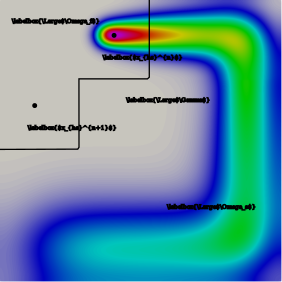
\includegraphics[width=\paperwidth,height=\paperheight]{transmission_conds/drawing.png}%
  }
  \begin{frame}[titleslide]
    \titlepage
  \end{frame}
  }

  \section{Introduction}
      \setbeamertemplate{frame footer}{\qquad Computational strategies for time-accurate simulation of part-scale \footlineHl{LPBF}}
  \subsection{Context: LPBF}
    \begin{frame}[sectionslide]
  \begin{center}
    \video<1>[above,autoplay,height=0.7,aspectratio=359/208,fit=contain]
\at (0.5,0.15) {videos/lpbf.mp4}
    % \begin{tikzpicture}[remember picture,overlay]
    %    \node[anchor=south west, inner sep=0pt] at (current page.south west) {%
    %      \movie[autostart] {\includegraphics[width=0.8\textwidth]{thumbnail-lpbf-section.png}}{videos/lpbf.mp4}%
    %    };
    % \end{tikzpicture}
  \end{center}
\end{frame}

\begin{frame}
  \frametitle{{LPBF}}
  \framesubtitle{MAM technology}
  Also known as PBF-LB/M (ISO nomenclature), one of the
  main Metal Additive Manufacturing (MAM) technologies

  \begin{figure}
    \begin{subfigure}[t]{0.32\textwidth}
      \centering
      \includegraphics[width=\linewidth]{waam.jpg}
      \textbf{Wire Arc Additive Manufacturing
      (\raisebox{-5pt}{\includegraphics[height=16pt]{waam-comic-effect.png}})}
    \end{subfigure}%
    \hfill
    \begin{subfigure}[t]{0.32\textwidth}
      \centering
      \includegraphics[width=\linewidth]{ded.jpg}
      \textbf{Directed Energy Deposition (DED)}
    \end{subfigure}%
    \hfill
    \begin{subfigure}[t]{0.32\textwidth}
      \centering
      \includegraphics[width=\linewidth]{lpbf.png}
      \textbf{Laser Powder Bed Fusion (LPBF)}
    \end{subfigure}
  \end{figure}
\end{frame}

\begin{frame}
  \frametitle{LPBF}
  % \framesubtitle{How does it work?}
  \begin{center}
    \video<1>[above,autoplay,height=0.7,aspectratio=16/9,fit=fill,controls]
\at (0.5,0.1) {videos/Build_chamber_process_animation.webm}
  \end{center}
\end{frame}

\begin{frame}
  \frametitle{{LPBF}}
  \framesubtitle{Fast, small, precise}

  \begin{table}
    \centering
    \begin{tabular}{l
      S
      S
      S }
      \toprule
      & {Radius $R$} 
      & {Speed $V$} 
      & {Power $P$} \\
      \midrule
      WAAM 
        & \qtyrange[]{2}{4}{\milli\meter}
        & \qtyrange[]{3}{10}{\milli\meter\per\second}
        & \qtyrange[]{5}{15}{\kilo\watt} \\
      DED 
        & \qtyrange[]{0.5}{1.5}{\milli\meter}
        & \qtyrange[]{5}{20}{\milli\meter\per\second}
        & \qtyrange[]{1}{4}{\kilo\watt} \\
      LPBF 
        & \qtyrange[]{25}{100}{\micro\meter}
        & \qtyrange[]{400}{1400}{\milli\meter\per\second}
        & \qtyrange[]{0.2}{1}{\kilo\watt} \\
      \bottomrule
    \end{tabular}
    \caption{Characteristic heat source parameters for the main MAM technologies.}
  \end{table}
  \vspace{-4mm}
  % LPBF offers a finer resolution and smoother surface finish,
  % but it is limited to smaller parts.
  \begin{figure}
    \centering
    \begin{subfigure}[t]{0.48\textwidth}
      \centering
      \includegraphics[width=0.74\linewidth]{waam-example.jpg}\\
      {\scriptsize WAAM: large parts (> \qty{1}{\meter}), coarse features.}
    \end{subfigure}%
    \hfill
    \begin{subfigure}[t]{0.48\textwidth}
      \centering
      \includegraphics[width=0.55\linewidth]{lpbf-fine.png}\\
      {\scriptsize LPBF: small part (< \qty{1}{\meter}), fine features.}
    \end{subfigure}
  \end{figure}

\end{frame}


    \setbeamertemplate{frame footer}{Computational strategies for time-accurate \footlineHl{simulation} of \footlineHl{part-scale} LPBF}
    \subsection{Multiscale \& multiphysics}
      \begin{frame}
  \frametitle{LPBF}
  \framesubtitle{Extremely multiscale}
  LPBF is an \textit{extremely multiscale} application \citep{hodge2021}.\\
  Let's quantify this statement:
  \begin{itemize}
    \item The \textbf{smallest} spatial and temporal \textbf{scales} are governed by the
      \textbf{heat source}, characterized by its radius $\mathbf{R}$ and by
      the time it takes to travel one radius,
      \[
        \mathbf{T_{hs}} := \frac{R}{V}.
      \]
    \item The \textbf{largest} spatial and temporal \textbf{scales} are set
      by the \textbf{part} and the printer.
      We choose here the characteristic part length $\mathbf{L_{part}}$ and
      the net printing time $\mathbf{T_{print}}$, i.e. the cumulative
      laser-on time.
  \end{itemize}
\end{frame}

\begin{frame}
  \frametitle{LPBF}
  \framesubtitle{Extremely multiscale}
  \centering
  \begin{minipage}{0.59\textwidth}
    \begin{figure}[ht]
      \def\svgwidth{0.84\columnwidth}
      \import{./figures/cube-example}{cube-scan-schematic.pdf_tex}
      \caption{Cube scan path of \textbf{side length} $L$, \textbf{layer thickness} $t$
      and \textbf{hatch spacing} $h$.}
    \end{figure}
  \end{minipage}%
  \hfill%
  \begin{minipage}{0.38\textwidth}
    \textbf{Space}:
    \begin{gather*}
      \text{Length scale ratio} = \frac{L}{R}\\
      \Large\Downarrow\\
      \alert<2>{\text{Volume scale ratio} = \frac{L^3}{R^3}}
    \end{gather*}
    \textbf{Time}:
    Assuming $h$ and $t$ are equal to $R$ for simplicity,
    \begin{gather*}
      T_{print} = \frac{L^3}{R^2 V}, \quad T_{hs} = \frac{R}{V}\\
      \Large\Downarrow\\
      \alert<2>{\text{Time scale ratio} = \frac{T_{print}}{T_{hs}} = \frac{L^3}{R^3}}
    \end{gather*}
  \end{minipage}
\end{frame}

% \begin{frame}
%   \frametitle{LPBF}
%   \framesubtitle{Extremely multiscale}
%   For this simple geometry, the net print time is
%   \begin{gather*}
%     T_{print} = N_{hatches} \cdot T_{hatch} = N_{layers} \cdot N_{hatches/layer} \cdot T_{hatch}\\
%     T_{hatch} = \frac{L}{V}\\
%     \implies
%     T_{print} = \frac{L}{R} \cdot \frac{L}{R} \cdot \frac{L}{V} = \frac{L^2}{R^2} \cdot \frac{L}{V} = \frac{L^3}{R^2 V}
%   \end{gather*}
%   Therefore, the time scale disparity is
%   $$
%   \frac{T_{print}}{T_{hs}} = \frac{L^3}{R^2 V} \cdot \frac{V}{R} = \left(\frac{L}{R}\right)^3
%   $$
% \end{frame}

\begin{frame}
  \frametitle{LPBF}
  \framesubtitle{Multiphysics}
  \begin{figure}
    \centering
    \includegraphics[height=0.8\textheight]{bayat2021.png}
    \caption{Relevant physics at melt-pool and part scales \citep{bayat2021}.}
    \label{fig:bayat2021}
  \end{figure}
\end{frame}


    \subsection{Part-scale aspirations}
      \begin{frame}
  \frametitle{Part-scale simulation}
  \framesubtitle{Why?}

  LPBF is both \textbf{extremely multiscale} and a \textbf{multiphysics} application.
  Despite this complexity, predictions are required at the \textbf{part scale}.

  \vspace{0.5em}
  Part-scale simulation aims to:
  \begin{itemize}
    \item Reduce costly experimental trial-and-error
    \item Predict residual stresses and part distortions
    \item Link thermal history to microstructure features
    \item Enable process-parameter optimization
    \item Shorten the design-to-manufacturing cycle
  \end{itemize}
\end{frame}

\begin{frame}
  \frametitle{Part-scale simulation}
  \framesubtitle{Problem statement}
  \begin{figure}[ht]
    \def\svgwidth{0.9\columnwidth}
    \hspace{-6mm}
    \import{./figures/lpbf_schematic}{schematic.pdf_tex}
    \caption{Schematic of the LPBF computational domain 
    $\Omega(t)$, encompassing the bulk (part and substrate) and powder bed regions,
    together with the applied heat source and convective/radiative heat losses.
  }
  \end{figure}
\end{frame}

\begin{frame}
  \frametitle{Part-scale simulation}
  \framesubtitle{PDE}
  {\small
  Define the extended temperature and liquid fraction fields
  \begin{equation*}
    T_e\dependson{\mathbf{x}, t} =
    \begin{cases}
      T\dependson{\mathbf{x}, t} & \mathbf{x} \in \overline{\Omega}(t)\\
      T_{dep} & \mathbf{x} \in \overline{\Omega}(t_{final}) \setminus \overline{\Omega}(t)
    \end{cases}
    \qquad
    f_{l,\; e}\dependson{\mathbf{x}, t} = f_l(T_e\dependson{\mathbf{x}, t})
  \end{equation*}
  where $T_{dep}$ is the deposition temperature.\\
  Find $T : \Omega(t) \times [0, T_{\text{final}}] \to \mathbb{R}$ such that
  \begin{align}
    \label{eq:original_pde}
    \rho c_p \partial_t T_e + \rho L \partial_t f_{l,\; e} - k \Delta T
    &= r\dependson{\mathbf{x}, t} &&\forall \mathbf{x} \in \Omega(t)\\
    \notag
    - k \partial_n T &= h_{conv} (T - T_{\text{env}}) + \varepsilon \sigma (T^4 - T_{\text{env}}^4) &&\forall \mathbf{x} \in \partial \Omega(t)\\
    \notag
    T\dependson{\mathbf{x}, 0} &= T_0 \qquad &&\forall \mathbf{x} \in \Omega(0)
  \end{align}
  }
    \todo{Comment on phase change treatment here}
\end{frame}

\begin{frame}
  \frametitle{Part-scale simulation}
  \framesubtitle{Discretization}
    Source-based latent heat treatment of \cite{celentano1994}:
    $f_l(T)$ is directly discretized in time.
    \begin{figure}
      \centering
      \begin{subfigure}[t]{0.33\textwidth}
        \begin{tikzpicture}
        \begin{axis}[
            xmin=-0.1, xmax=1.1,
            ymin=+0, ymax=1.1,
            axis lines=center,
            axis on top=true,
            ytick={0, 1},
            xtick={0.05, 0.95},
            xticklabels={$T_s$, $T_l$},
            domain=-0.1:1.1,
            ylabel=$f_l$,
            xlabel=$T$,
            %legend style={at={(0.03,0.5)},anchor=west},
            height=0.4\pageheight
            ]

            \def\Ts{0.05}
            \def\Tl{0.95}
            \newcommand{\flalpha}[1]{2*#1/(\Tl - \Ts)}
            \newcommand{\fl}[1]{
              0.5*(tanh(\flalpha{#1}*(\x - 0.5))+1)
            }
            \addplot+ [mark=none, ultra thick, smooth] {\fl{1}};
            \addplot+ [mark=none, ultra thick, smooth] {\fl{2}};
            \addplot+ [mark=none, ultra thick, smooth] {\fl{4}};
            
            %% Add the asymptotes
            \draw [blue, dotted, thick] (axis cs:+1.1,+1)-- (axis cs:0,+1);
        \end{axis}
        \end{tikzpicture}
      \end{subfigure}%
      \hfill
      \begin{subfigure}[t]{0.33\textwidth}
        \begin{tikzpicture}
        \begin{axis}[
            xmin=-0.1, xmax=1.1,
            ymin=+0, ymax=4.5,
            axis lines=center,
            axis on top=true,
            ytick={0},
            xtick={0.05, 0.95},
            xticklabels={$T_s$, $T_l$},
            domain=-0.1:1.1,
            ylabel=$f_l'$,
            legend style={at={(0.7,0.8)},anchor=west},
            height=0.4\pageheight
            ]

            \def\Ts{0.05}
            \def\Tl{0.95}
            \newcommand{\flalpha}[1]{2*#1/(\Tl - \Ts)}
            \newcommand{\flp}[1]{
              \flalpha{#1}/2*(1 - (tanh(\flalpha{#1}*(\x - 0.5)))^2)
            }
            \addplot+ [mark=none, ultra thick, smooth] {\flp{1}};
            \addlegendentry{$S = 1$}                
            \addplot+ [mark=none, ultra thick, smooth] {\flp{2}};
            \addlegendentry{$S = 2$}                
            \addplot+ [mark=none, ultra thick, smooth] {\flp{4}};
            \addlegendentry{$S = 4$}
            
        \end{axis}
        \end{tikzpicture}
      \end{subfigure}%
      \hfill
      \begin{subfigure}[t]{0.33\textwidth}
        \begin{tikzpicture}
        \begin{axis}[
            xmin=-0.1, xmax=1.1,
            ymin=-4, ymax=4,
            axis lines=center,
            axis on top=true,
            ytick={0},
            xtick={0.05, 0.95},
            xticklabels={$T_s$, $T_l$},
            domain=-0.1:1.1,
            ylabel=$f_l''$,
            height=0.4\pageheight
            ]

            \def\Ts{0.05}
            \def\Tl{0.95}
            \newcommand{\flalpha}[1]{2*#1/(\Tl - \Ts)}
            \newcommand{\flpp}[1]{
              \flalpha{#1}^2*tanh(\flalpha{#1}*(\x - 0.5))*((tanh(\flalpha{#1}*(\x - 0.5)))^2 - 1)
            }
            \addplot+ [mark=none, ultra thick, smooth] {\flpp{1}};
            \addplot+ [mark=none, ultra thick, smooth] {\flpp{2}};
            \addplot+ [mark=none, ultra thick, smooth] {\flpp{4}};
            
        \end{axis}
        \end{tikzpicture}
      \end{subfigure}
      \caption{Liquid fraction $f_l$ and derivatives.}
      \label{fig:fl_fld_fldd}
    \end{figure}
    Multiply \cref{eq:original_pde}
    by $\phi \in V_T(t) = H^{1}\left(\Omega(t)\right)$;
    integrate over $\Omega\dependson{t}$;
    apply integration by parts on the diffusion term; insert BCs;
    apply BDF1
    {\small
    \begin{gather*}
      \label{eq:weak_heat}
      \int_{\Omega} \phi \rho \left({c_p \frac{T^{n+1} - T^n}{\Delta t} + L \frac{f_l(T^{n+1}) - f_l(T^n)}{\Delta t}}\right)
      + \int_{\Omega} \nabla \phi \cdot \left(k \nabla T\right)\\
      \notag
      \forall \phi \in V_T(t) \hspace{1cm}
      \;=\; \int_{\Omega} \phi r
      + \int_{\partial \Omega} \phi \left({h_{\text{conv}} \left( T - T_{\text{env}} \right)
      + \varepsilon \sigma \left( {T}^4 - T_{\text{env}}^4 \right)}\right)
    \end{gather*}
    }

\end{frame}

\begin{frame}
  \frametitle{Part-scale simulation}
  \framesubtitle{Discretization}
  \begin{figure}
    \begin{subfigure}[t]{0.33\textwidth}
      \includegraphics[height=0.35\pageheight]{schematic_melting/0.png}
      \caption{Bare substrate below an inactive powder layer.}
      \label{fig:refModelBareSubstrate}
    \end{subfigure}\hfill%
    \begin{subfigure}[t]{0.33\textwidth}
      \includegraphics[height=0.35\pageheight]{schematic_melting/1.png}
      \caption{A powder layer is activated during a recoating step.}
      \label{fig:powderLayer}
    \end{subfigure}\hfill%
    \begin{subfigure}[t]{0.33\textwidth}
      \includegraphics[height=0.35\pageheight]{schematic_melting/2.png}
      \caption{After a heating step, elements whose average temperature
      surpasses $T_m$ are set to bulk.}
      \label{fig:activPhaseChange3}
    \end{subfigure}\hfill%
    \caption{Illustration of deposition and melting processes.\qquad
      \legendpowderbulk{}
    }
    \label{fig:activPhaseChange}.
  \end{figure}
  Same treatment of phase change as in \citep{kollmannsberger2018}
\end{frame}

\begin{frame}
  \frametitle{Part-scale simulation}
  \framesubtitle{Demo video}

  \begin{figure}
    \video<1>[above,height=0.7,aspectratio=62/27,fit=fill,controls]
  at (0.5,0.18) {videos/2dlpbf_2d_lpbf_ref.mp4}
    \vspace{0.7\pageheight+3pt}
    \videoCaption{
      Demo simulation of 2D LPBF with element activation.\\
      Wireframe elements (\;\wireframeTriangle{}) correspond to powder region.
    }
  \end{figure}

\end{frame}


    \setbeamertemplate{frame footer}{Computational strategies for \footlineHl{time-accurate} simulation part-scale LPBF}
    \subsection{Impossible!}
      \begin{frame}
  \frametitle{Part-scale simulation}
  \framesubtitle{Impossible}
  Previous slide: ``uniform'' mesh in part and powder region.
  Recall the volume scale ratio;
  In 3D, we would need
  \begin{equation}
    \label{eq:num_elements_uniform_mesh}
    \text{\# elements} = \mathcal{O}\left(\frac{L^3}{R^3}\right)
  \end{equation}
  to resolve the heat source throughout the print.

  In practice, no one uses uniform meshes for LPBF simulation;
  \textbf{AMR} is regarded as the \textbf{de facto standard}.
\end{frame}

\begin{frame}
  \frametitle{Part-scale simulation}
  \framesubtitle{Impossible}
  But what about time-steps?
  The interval of interest is $]0, T_{final}[$ with
  $$
  T_{final} = T_{print} + T_{cool}
  $$
  i.e. the net printing time plus cooling.
  The time scale disparity requires again \cref{eq:num_elements_uniform_mesh} time-steps
  \begin{gather*}
    \label{eq:num_timesteps_uniform_mesh}
    \text{\# time-steps} > \frac{T_{print}}{T_{hs}} = \mathcal{O}\left(\frac{L^3}{R^3}\right)
  \end{gather*}
  when discretizing with \textbf{uniform time-steps}.
\end{frame}

\begin{frame}
  \frametitle{Part-scale simulation}
  \framesubtitle{Impossible}
  Intuitively, if we don't respect the constraint
  \begin{equation}
    \label{eq:origconstraint}
    \Delta t \leq T_{hs},
  \end{equation}
  we won't resolve the motion of the heat source.\\
  In practice, that's indeed what happens:
  if the time-step is larger than $T_{hs}$ i.e. the heat source
  travels more than $1 R$ per time-step,
  it skips over parts of the domain,
  and generates artificial temperature spikes.
  \begin{figure}
    \begin{subfigure}[t]{0.49\textwidth}
      \includegraphics[width=\textwidth]{timestep-2ths/1R.png}
      \caption{$\Delta t = 1 T_{hs}$}
      \label{fig:spots1R}
    \end{subfigure}
    \begin{subfigure}[t]{0.49\textwidth}
      \includegraphics[width=\textwidth]{timestep-2ths/2R.png}
      \caption{$\Delta t = 2 T_{hs}$}
      \label{fig:spots2R}
    \end{subfigure}
    % \caption{2D heating track example with admissible and inadmissible
    % time-step sizes according to inequality \eqref{eq:origconstraint}.}
    % \label{fig:spots}
  \end{figure}
\end{frame}

\begin{frame}
  \frametitle{Part-scale simulation}
  \framesubtitle{Impossible}
  So \eqref{eq:num_timesteps_uniform_mesh} is indeed a \textbf{lower bound} on the number of time-steps
  when using uniform time-stepping.

  \underline{Bad news:}
  \begin{itemize}
    \item \textbf{Uniform time-stepping} is the \textbf{de facto standard} in LPBF simulation.
    \item Some references require time-steps much smaller than $T_{hs}$
      to ensure stability and accuracy \citep{hodge2014, hodge2021, elahi2025}.
  \end{itemize}
  There are basically 4 (!) groups in the world that can run simulations in the order of \textbf{centimeters}:
  Pittsburgh, Northwestern, LLNL, TUM.\\
  \textbf{Decimeter}-scale parts are currently unfeasible.
  \todo{Expand}
\end{frame}

\begin{frame}
  \frametitle{Part-scale simulation}
  \framesubtitle{Lumped heat source}
  
  What do you do if you don't have a cluster or a nice GPU ?
  You \textbf{simplify the model}.

  \begin{figure}
    \centering
    \begin{tikzpicture}
      % include the original figure
      \node[inner sep=0] (img) {\def\svgwidth{0.3\textwidth}%
        {\small \import{./figures/goldakProfile}{profile.pdf_tex}}};

      % red "forbidden" cross over the whole image (hidden on overlay 1)
      \uncover<2>{
        \draw[line width=2pt, red] ([shift={(-2mm,-2mm)}]img.south west)
                                   -- ([shift={(+2mm,+2mm)}]img.north east);
        \draw[line width=2pt, red] ([shift={(+2mm,-2mm)}]img.south east)
                                   -- ([shift={(-2mm,+2mm)}]img.north west);
      }
    \end{tikzpicture}
    \caption{Double ellipsoidal profile \citep{goldak1984}.
      $\xi$ is the welding direction.}
    \label{fig:goldak}
  \end{figure}

  \uncover<2>{
    We give up on the accurate representation of the heat source
    since it is too costly to resolve.

    We use a \textbf{lumped heat source} instead.
  }
\end{frame}

\begin{frame}
  \frametitle{Part-scale simulation}
  \framesubtitle{Lumped heat source}
  A time-step is chosen regardless of the heat source path.
  Elements that are intersected by the heat source path
  during the time-step are \textbf{heated uniformly}.
  \begin{figure}
    \centering
    \begin{subfigure}[t]{0.495\textwidth}
      \centering
      \def\svgwidth{\textwidth}
      \import{./figures/lumped_hs}{heated_els.pdf_tex}
      \caption{Elements heated uniformly during $[t^{n},\,t^{n+1}]$.\\
           \begin{tikzpicture}
             \draw[red, very thick, dashed] (0,0.3) -- (0.4,0.3);
           \end{tikzpicture}
           $\; \rightarrow \;$ Heat source path
         }
      \label{fig:lhs_heated_els}
    \end{subfigure}%
    \hfill%
    \begin{subfigure}[t]{0.48508\columnwidth}
      \centering
      \includegraphics[width=\textwidth]{lumped_hs/tem.png}
      \caption{Resulting temperature field.}
      \label{fig:lhs_temp_field}
    \end{subfigure}
    \caption{Lumped heat source example.}
  \end{figure}
\end{frame}

\begin{frame}
  \frametitle{Part-scale simulation}
  \framesubtitle{Lumped heat source}
  \begin{figure}
    \begin{subfigure}[t]{0.32\textwidth}
      \centering
      \includegraphics[width=\textwidth]{chiumenti2017-lhs/chiumenti2017multipleHatches.png}
      \caption{Multiple hatches per time-step.}
    \end{subfigure}%
    \hfill
    \begin{subfigure}[t]{0.32\textwidth}
      \centering
      \begin{tikzpicture}[
        spy using outlines= {connect spies}
      ]
        \node[inner sep=0] (img) {\includegraphics[width=\textwidth]{chiumenti2017-lhs/chiumenti2017singleLayer.png}};
        \coordinate (spypoint) at ($(img.south west)!.88!(img.south east)!0.325!(img.north east)$);
        \coordinate (magnifypoint) at ($($(img.south west)!.5!(img.south east)$)!.2!($(img.north west)!.5!(img.north east)$)$);

        \only<2->{
          \spy [black, width=2cm, height=1cm, magnification=2.5] on (spypoint) in node[fill=white] at (magnifypoint);
        }
      \end{tikzpicture}
      \caption{Single layer per time-step.}
    \end{subfigure}%
    \hfill
    \begin{subfigure}[t]{0.32\textwidth}
      \centering
      \includegraphics[width=\textwidth]{chiumenti2017-lhs/chiumenti2017multipleLayers.png}
      \caption{4 layers per time-step.}
    \end{subfigure}
    \caption{Lumped heat input strategies from \cite{chiumenti2017b}.}
  \end{figure}
  \vspace{-5mm}
  \textit{Pros and cons}
  \begin{itemize}
    \item[+] Feasible simulations
    \uncover<2->{\item[-] Distributed heat input $\;\longrightarrow\;$ temperatures below melt $\;\longrightarrow\;$ Numerical calibration (flash heating)}
    \uncover<2->{\item[-] Loss of history: no resolution of heat source motion}
  \end{itemize}
\end{frame}



  \setbeamertemplate{frame footer}{\footlineHl{Computational strategies for time-accurate simulation part-scale LPBF}}
  \section{Objectives}
    \begin{frame}
  \frametitle{Problematic}
  \begin{itemize}
    \item AMR is regarded as necessary for part-scale LPBF simulation
      to adress spatial scale disparity.
    \item The time scale disparity is \textbf{equally} severe,
      yet uniform-time stepping is the standard.
  \end{itemize}
  $\implies$ Largely overlooked challenge:
  reduce the number of global time-steps required
  in part-scale LPBF simulation
  while retaining time-accuracy.
\end{frame}

\begin{frame}
  \frametitle{Objectives of this work}
  \begin{itemize}
    \item
      Review existing methods for addressing time-stepping
      challenges in MAM.
    \item
      Explore novel methods for reducing the number of time-steps
      required in LPBF modeling.
    \item
      Validate the proposed methods on realistic
      test cases.
    \item
      Validate the underlying physical models
      and numerical methods against experimental data.
    \item
      Provide realistic speedup estimates and practical implementation guidelines
      for the proposed methods.
    \item Ensure open science and reproducibility.
  \end{itemize}
\end{frame}



  \setbeamertemplate{frame footer}{}

  \section{Domain decomposition}
    \begin{frame}
  \centering
  \begin{tikzpicture}[
    font=\small,
    box/.style={draw, rounded corners, align=center, inner sep=6pt},
    arr/.style={->, thick}
  ]

  \node[box] (ms) {LPBF multiscale constraints};

  \node[box, below=5mm of ms] (dd) {Domain decomposition\\(core framework)};

  \node[box, below left=4mm and 4mm of dd] (as) {Advected subdomain\\\citep{slimani2024}};

  \node[box, below right=4mm and 4mm of dd] (ss) {Substepping\\\citep{slimani2025}};

  \draw[arr] (ms) -- (dd);
  \draw[arr] (dd) -- (as);
  \draw[arr] (dd) -- (ss);

  \end{tikzpicture}
\end{frame}

\begin{frame}
  \frametitle{Domain decomposition}
  \framesubtitle{Basics}
  We've established that the part-scale build is driven
  by the motion of a very localized heat source.

  What if we treat differently this region aka the Heat Affected Zone (HAZ)?

  We will do so via \textbf{domain decomposition} (DD).

  Let $\Omega_1$ and $\Omega_2$ be a non-overlapping decomposition of
  the domain $\Omega = \Omega_1 \sqcup \Omega_2$ such that
  $\Omega_1$ contains the HAZ;
  we will pose different problems in $\Omega_1$ and $\Omega_2$
  and enforce \textbf{transmission conditions} at the interface
  $\Gamma = \partial \Omega_1 \cap \partial \Omega_2$
\end{frame}

\begin{frame}
  \frametitle{Domain decomposition}
  \framesubtitle{Basics}
\begin{figure}
  \centering
  \def\svgwidth{1.0\columnwidth}
  \import{figures/transmission_conds/}{drawing.pdf_tex}
  \caption{Non-overlapping DD schematic for a welding problem. $\Omega_1$ and $\Omega_2$
  cover the HAZ and underlying substrate, respectively. Transmission conditions
  must be satisfied at the interface $\Gamma = \partial \Omega_1 \cap \partial \Omega_2$.
  Admissible and inadmissible transmission conditions are shown in the miniature plots,
  which represent temperature fields across $\Gamma$.
  }
  \label{fig:transmission_conditions}
\end{figure}
\end{frame}

\begin{frame}
  \frametitle{Domain decomposition}
  \framesubtitle{Basics}
  Consider the linear heat equation with Dirichlet boundary conditions.
  Solve for $T_i$ in each subdomain $\Omega_i$:
  \begin{equation}
  \label{eq:lproblem}
  \left\{
  \begin{aligned}
    \partial_t T_i - \alpha \Delta T_i &= r && \forall \mathbf{x} \in \Omega_i\\
    T_i(\mathbf{x}, t) &= T_d && \forall \mathbf{x} \in \partial \Omega_{D,i}\\
    \mathcal{I}_i \left(T_i, T_j\right) &= 0 && \forall \mathbf{x} \in \Gamma, \enskip i \neq j
  \end{aligned}
  \right.
  \end{equation}
  This is equivalent to solving the original problem in $\Omega$ given
  that the \textbf{transmission conditions}
  are satisfied
  \begin{equation}
    \label{eq:interface_eq_conditions}
    \begin{cases}
      \mathcal{I}_1(T_1, T_2) = 0\\
      \mathcal{I}_2(T_1, T_2) = 0
    \end{cases}
    \iff
    \begin{cases}
      T_1 = T_2\\
      k_1 \partial_n T_1 = k_2 \partial_n T_2
    \end{cases}
    \qquad
    \qquad
    \forall \mathbf{x} \in \Gamma
  \end{equation}
\end{frame}

\begin{frame}
  \frametitle{Domain decomposition}
  \framesubtitle{Basics}
  Any linearly independent combination of \eqref{eq:interface_eq_conditions}
  lays a valid pair of subproblems on $\Omega_1$ and $\Omega_2$
  {\small
  \begin{equation}
    \label{eq:lp1}
    \left\{
    \begin{aligned}
      \rho c_p \partial_t T_1 - k \Delta T_1 &= r && \text{ in } \Omega_1\\
      T_1 &= T_d && \text{ in } \partial \Omega_{D,1}\\
      \gamma_1 T_1 + \eta_1 k_1 \frac{\partial T_1}{\partial n_1} &= \gamma_1 T_2 + \eta_1 k_2 \frac{\partial T_2}{\partial n_1} && \text{ in } \Gamma
    \end{aligned}
    \right.
  \end{equation}
  \begin{equation}
    \label{eq:lp2}
    \left\{
    \begin{aligned}
      \rho c_p \partial_t T_2 - k \Delta T_2 &= r && \text{ in } \Omega_2\\
      T_2 &= T_d && \text{ in } \partial \Omega_{D,2}\\
      \gamma_2 T_2 + \eta k_2 \frac{\partial T_2}{\partial n_2} &= \gamma_2 T_2 + \eta_2 k_2 \frac{\partial T_2}{\partial n_2} && \text{ in } \Gamma
    \end{aligned}
    \right.
  \end{equation}
  }
  \begin{itemize}
    \item $\gamma_1 = \eta_2 \neq 0$ and $\gamma_2 = \eta_1 = 0 \longrightarrow\;$ Dirichlet-Neumann

    \item $\gamma_i \neq 0$ and $\eta_i \neq 0 \longrightarrow\;$ Robin-Robin

    \item $\gamma_1 \neq 0$, $\eta_1 = 0$, $\gamma_2 \neq 0$ and $\eta_2 \neq 0
      \longrightarrow\;$ Dirichlet-Robin
  \end{itemize}
\end{frame}

\begin{frame}
  \frametitle{Domain decomposition}
  \framesubtitle{Basics}
  Assuming steady-state and applying FEM discretization
  on both subdomains, we obtain the following
  monolithic system:
  \renewcommand{\arraystretch}{1.2} % increases spacing (default is 1.0)
  \begin{equation}
    \label{eq:monolithic}
    \begin{pmatrix}
      \mathbf{A}_{11} & \mathbf{A}_{1\Gamma_1} & \cdot & \cdot\\
      \mathbf{A}_{\Gamma_1 1} & \mathbf{A}_{\Gamma_1 \Gamma_1} + \mathbf{R}_{11} & \cdot & \mathbf{R}_{12}\\
      \cdot & \cdot & \mathbf{A}_{22} & \mathbf{A}_{2\Gamma_2}\\
      \cdot & \mathbf{R}_{21} & \mathbf{A}_{\Gamma_2 2} & \mathbf{A}_{\Gamma_2 \Gamma_2} + \mathbf{R}_{22}
    \end{pmatrix}
    \begin{pmatrix}
      \mathbf{T}_1\\
      \mathbf{T}_{\Gamma_1}\\
      \mathbf{T}_2\\
      \mathbf{T}_{\Gamma_2}
    \end{pmatrix}
    =
    \begin{pmatrix}
      \mathbf{F}_1\\
      \mathbf{F}_{\Gamma_1}\\
      \mathbf{F}_2\\
      \mathbf{F}_{\Gamma_2}
    \end{pmatrix}
  \end{equation}
  $$
      \underbrace{\int_{\Omega_i} \nabla v_i \cdot k \nabla T_i}_{\mathbf{A}}\,
    - \underbrace{\int_{\Gamma} v_i \gamma_i T_i}_{\mathbf{R}_{ii}}\,
    = \underbrace{\int_{\Omega_i} r v_i\,}_{\mathbf{F}}\,
    - \underbrace{\int_{\Gamma} v_i \left(\gamma_i T_j + \eta_i k \partial_n T_j\right)}_{\mathbf{R}_{ij}}
  $$
  Solving \eqref{eq:monolithic} directly $\; \longrightarrow\;$ \textbf{monolithic} approach
\end{frame}

\begin{frame}
  \frametitle{Domain decomposition}
  \framesubtitle{Basics}
  
  Solving problem on $\Omega_1$
  \renewcommand{\arraystretch}{1.2} % increases spacing (default is 1.0)
  \begin{equation}\label{eq:staggered1}
    \begin{pmatrix}
      \mathbf{A}_{11} & \mathbf{A}_{1\Gamma_1}\\
      \mathbf{A}_{\Gamma_1 1} & \mathbf{A}_{\Gamma_1 \Gamma_1} + \mathbf{R}_{11}
    \end{pmatrix}
    \begin{pmatrix}
      \mathbf{T}^{k+1}_1\\
      \mathbf{T}^{k+1}_{\Gamma_1}
    \end{pmatrix}
    =
    \begin{pmatrix}
      \mathbf{F}_1\\
      \mathbf{F}_{\Gamma_1} - \mathbf{R}_{12} \mathbf{T}^k_{\Gamma_2}
    \end{pmatrix}
  \end{equation}
  and feeding the interface values to the problem on $\Omega_2$
  \begin{equation}\label{eq:staggered2}
    \begin{pmatrix}
      \mathbf{A}_{22} & \mathbf{A}_{2\Gamma_2}\\
      \mathbf{A}_{\Gamma_2 2} & \mathbf{A}_{\Gamma_2 \Gamma_2} + \mathbf{R}_{22}
    \end{pmatrix}
    \begin{pmatrix}
      \mathbf{T}^{k+1}_2\\
      \mathbf{T}^{k+1}_{\Gamma_2}
    \end{pmatrix}
    =
    \begin{pmatrix}
      \mathbf{F}_2\\
      \mathbf{F}_{\Gamma_2} - \mathbf{R}_{21} \mathbf{T}^{k+1}_{\Gamma_1}
    \end{pmatrix}
  \end{equation}
  \renewcommand{\arraystretch}{1.0}
  and iterating until convergence $\; \longrightarrow\;$ \textbf{staggered} approach
\end{frame}



  \section{Advected subdomain}
    \subsection{Introduction}
  \begin{frame}
  \frametitle{Advected subdomain}
  Resolving the motion requires prohibitively small time-steps.

  Idea: \textbf{Get rid of the motion}!

  Define a subdomain $\Omega_m$ that moves with the heat source
  and solves the heat equation in its reference frame.

  Due to motion of reference frame, the heat equation in $\Omega_m$
  acquires an advection term $\longrightarrow$ \textbf{advected subdomain}
  (AS) method.
\end{frame}


\subsection{Method}
  \begin{frame}
  \frametitle{Advected subdomain}
  \begin{figure}
    \centering
    \def\svgwidth{1.05\columnwidth}
    \small
    \import{./figures/chimera_schematic/}{chimera_schematic.pdf_tex}
    \caption{Schematic of Robin-Robin variant of advected subdomain method.}
    \label{fig:chimera_schematic}
  \end{figure}
\end{frame}

\begin{frame}
  \frametitle{Advected subdomain}

    {\small
    \begin{gather*}
      (\mathbf{x}, t) \longrightarrow (\boldsymbol{\xi}, \eta) \thinspace , \thinspace
      \begin{cases}
        \boldsymbol{\xi} = \mathbf{x} - \int_0^t \mathbf{v}\dependson{t} dt\\
        \eta = t
      \end{cases}
    \end{gather*}
    \begin{gather*}
      \Longrightarrow
      \begin{cases}
        \partial_{x_i} &= \partial_{\xi_i} \Rightarrow \nabla_{\mathbf{x}} = \nablaxi\\
        \partial_t &= \partial_\eta - v_i \partial_{\xi_i} = \partial_\eta - \mathbf{v}\dependson{t} \cdot \nablaxi
      \end{cases}
    \end{gather*}

    Find $T_m : \Omega_m(t) \times [0, T_{\text{final}}] \to \mathbb{R}$
    and $T_f : \Omega_f(t) \times [0, T_{\text{final}}] \to \mathbb{R}$
    such that
    \begin{align*}
      \rho c_p \Big( \partial_t T^m{\scriptstyle (\xi, t)} - \mathbf{v}\dependson{t} \cdot \nabla T^m{\scriptstyle (\xi, t)} \Big) -
      \nabla \cdot ( k \nabla T^m{\scriptstyle (\xi, t)}) &= r{\scriptstyle (\xi)}  &\xi &\in \Omega_m(t)
    \end{align*}
    \begin{align*}
    \rho c_p \partial_t T^f{\scriptstyle (x, t)} - \nabla \cdot (k \nabla T^f{\scriptstyle (x, t)}) &= 0 \qquad &x &\in \Omega_f(t)
    \end{align*}
    }
\end{frame}

\begin{frame}
  \frametitle{Advected subdomain}
  \cite{slimani2024}: Dirichlet-Neumann multi-mesh variant of advected
  subdomain method for linear heat equation.
  \begin{figure}[h]
    \centering
    \includegraphics[width=0.6\textwidth]{quadTriang.png}
    \caption{A finer mesh can be attached to the heat source
    to adress spatial scale disparity: not done here.}
  \end{figure}
  \begin{itemize}
    \item VMS stabilization to handle advection in $\Omega_m$
    \item Monolithic solution of the coupled problem
    \item Serial C++ implementation available on GitHub.
  \end{itemize}
\end{frame}

\begin{frame}
  \frametitle{Advected subdomain}
  \framesubtitle{Growing $\Delta t$ workflow}
  We shifted the motion of the heat source into $\Omega_m$;
  the time-scale of the motion is no longer $T_{hs}$,
  it is $T_{\Omega_m}$:
  $$
    T_{\Omega_m} := \frac{L_{\Omega_m}}{V} > T_{hs} \quad \text{ given } \quad L_{\Omega_m} > R
  $$
  \begin{itemize}
    \item $L_{\Omega_m}$ can be chosen and changed at each time-step.
    \item The PDE in $\Omega_m$ can admit a steady solution,
          provided that the geometry and material composition
          remain constant over a time interval.
  \end{itemize}
  $\longrightarrow$ \textbf{Growing} $\Delta t$ \textbf{workflow}\;:
  at the end of a time-step:

  \begin{center}
  \begin{tikzpicture}[node distance=1em, every node/.style={align=center}]
    \tikzset{
      blockdiagr/.style={
        draw,
        rounded corners,
        align=center,
        inner sep=4pt
      }
    }
    \node[blockdiagr] (metric) {$\texttt{steadiness\_metric}(T_m) < \epsilon$};
    \node[blockdiagr, below=of metric] (dt) {Increase $\Delta t$ for $t^{n+2} = t^{n+1} + \Delta t$};
    \node[blockdiagr, below=of dt] (omega) {Resize $\Omega_m$};
    \draw[->] (metric) -- (dt);
    \draw[->] (dt) -- (omega);
  \end{tikzpicture}
  \end{center}
  % where \texttt{steadiness\_metric} can be chosen as e.g.
  % $$
  % \max_{\Omega_m} \left| \frac{T_m^{n+1} - T_m^{n}}{\Delta t} \right|
  % \quad
  % \text{or}
  % \quad
  % \frac{\|T_m\big|_{t^{n+1}} - T_m\big|_{t^{n}}\|}{\|T_m\big|_{t^{n+1}}\|} 
  % $$
\end{frame}

\begin{frame}
  \frametitle{Advected subdomain}
  \framesubtitle{Workflow}
  \begin{columns}
    \begin{column}{0.4\textwidth}
      \begin{itemize}
      \item Dynamic resizing of $\Omega_m$\\
        $\longrightarrow$ background mesh
      \item $\Omega_m(t^n),\Omega_m(t^{n+1})\subset\Omega$\\
        $\longrightarrow$ \texttt{intersect} at $t^n$ and $t^{n+1}$
      \item Sizing of $\Omega_m$:
        \begin{itemize}
          \item Front and side lengths larger than $2 R$
            to contain support of heat source.
          \item Back length larger than $V \cdot \Delta t$
            to not skip regions of domain.
        \end{itemize}
      \end{itemize}
    \end{column}%
    \begin{column}{0.6\textwidth}
      \begin{figure}
        \begin{subfigure}[t]{0.49\columnwidth}
          \includegraphics[height=0.34\pageheight]{2d_meshing_example/afterShaping.png}
          \caption{$\mathcal{T}^m \leftarrow \texttt{shapeSubdomain}(\mathcal{T}^m_{bg})$}
        \end{subfigure}%
        \hfill%
        \begin{subfigure}[t]{0.49\columnwidth}
          \includegraphics[height=0.34\pageheight]{2d_meshing_example/after_intersec1.png}
          \caption{$\mathcal{T}^m \leftarrow \texttt{intersect}\big(\mathcal{T}^m, \mathcal{T}^f \textrm{ at } t^n\big)$}
        \end{subfigure}\\
        \begin{subfigure}[t]{0.49\columnwidth}
          \includegraphics[height=0.34\pageheight]{2d_meshing_example/after_intersec2.png}
          \caption{$\mathcal{T}^m \leftarrow \texttt{intersect}\big(\mathcal{T}^m, \mathcal{T}^f\big) \textrm{ at } t^{n+1}$}
        \end{subfigure}%
        \hfill%
        \begin{subfigure}[t]{0.49\columnwidth}
          \includegraphics[height=0.34\pageheight]{2d_meshing_example/dd.png}
          \caption{$\mathcal{T}^f \leftarrow \texttt{subtract}\big(\mathcal{T}^f, \mathcal{T}^m\big)$}
        \end{subfigure}
        \label{fig:2d_meshing_example}
      \end{figure}
    \end{column}%
  \end{columns}
\end{frame}



\subsection{Results (Slimani \& al. (2024))}
  \subsectiontoc{}
  \begin{frame}
  \frametitle{Advected subdomain}
  Analytical validation with 3D welding example
  \citep{nguyen1999,vanelsen2007}
  and Ti64-like material properties.
  \vspace{-5mm}
  \begin{figure}[]
      \centering
      \begin{tabular}{cc}
  \begin{subfigure}[t]{0.49\linewidth}
    \centering
    \includegraphics[width=\textwidth]{3d_weldingLpbf/analytical.png}
    \caption{Analytical}
  \end{subfigure} &
  \addtocounter{subfigure}{2}
  \begin{subfigure}[t]{0.49\linewidth}
    \centering
    \includegraphics[width=\textwidth]{3d_weldingLpbf/allContours.png}
    \definecolor{referenceColor}{HTML}{1762FB}
    \definecolor{proposedColor}{HTML}{00AA00}
    \vspace{-0.7cm}
    \caption{
         ({\color{black} \rule[-1.5 pt]{8 pt}{8 pt}}) Analytical \;\;
         ({\color{proposedColor} \rule[-1.5 pt]{8 pt}{8 pt}}) AS \;\;
         ({\color{referenceColor} \rule[-1.5 pt]{8 pt}{8 pt}}) Reference \;\;
         \\
      Isothermals and position of maximum temperature.
    }
    \label{fig:3dweldallcontours}
  \end{subfigure} \\
  \addtocounter{subfigure}{-3}
  \begin{subfigure}[t]{0.49\linewidth}
    \centering
    \includegraphics[width=\textwidth]{3d_weldingLpbf/coupled_elsPerRad8.png}
    \caption{Advected subdomain (AS), $\Delta t = 2\,T_{hs}$}
    \label{fig:3dweldcontourprop}
  \end{subfigure} & 
  \addtocounter{subfigure}{2}
  \begin{subfigure}[t]{0.49\linewidth}
    \centering
    \includegraphics[width=\textwidth]{3d_weldingLpbf/err_coupled_elsPerRad8.png}
    \caption{Pointwise error of \ref{fig:3dweldcontourprop}. Max error is $\approx \mathbf{12}$}
  \end{subfigure} \\
  \addtocounter{subfigure}{-3}
  \begin{subfigure}[t]{0.49\linewidth}
    \centering
    \includegraphics[width=\textwidth]{3d_weldingLpbf/reference_elsPerRad8_tstepsPerRad4.png}
    \caption{Reference method, $\Delta t = 0.25\,T_{hs}$}
    \label{fig:3dweldcontourref}
  \end{subfigure} & 
  \addtocounter{subfigure}{2}
  \begin{subfigure}[t]{0.49\linewidth}
    \centering
    \includegraphics[width=\textwidth]{3d_weldingLpbf/err_reference_elsPerRad8_tstepsPerRad4.png}
    \caption{Pointwise error of \ref{fig:3dweldcontourref}. Max error is $\approx \mathbf{263}$}
    \label{fig:3dweldpointwiseref}
  \end{subfigure} \\
      \end{tabular}
    \caption{Solution (left) and error (right) contour at steady-state.}
  \end{figure}
\end{frame}

\begin{frame}
  \frametitle{Advected subdomain}
  \framesubtitle{2D welding example}
    \begin{figure}
      \centering
      \video<1>[above,height=0.7,aspectratio=1540/782,fit=contain,controls]
  at (0.5,0.15) {videos/chimera.mp4}
      \vspace{0.7\pageheight + 7pt}
      \videoCaption{
        \begin{tabular}{lc}
          Left & AS with growing $\Delta t$ workflow.\\
          Right & No AS, $\Delta t = 0.5 T_{hs}$.
        \end{tabular}
      }
    \end{figure}
\end{frame}

\begin{frame}
  \frametitle{Advected subdomain}
  \framesubtitle{Shearing!}

  \begin{figure}
    \centering
    \begin{subfigure}[t]{0.3\linewidth}
      \centering
      \stackinset{l}{ 0.35\textwidth}{b}{ 0.025\textwidth}{
        {\color{white}$\Omega_f$}
      }{
        \includegraphics[width=\textwidth]{2d_welding_chimera/changeOfDir_OFF.png}
      }
      \caption{No AS, $\Delta t = 0.5\,T_{hs}$.}
      \label{fig:2dWeldNoShear}
    \end{subfigure}
    \hfill
    \begin{subfigure}[t]{0.3\linewidth}
      \centering
      \stackinset{r}{ 0.32\textwidth}{b}{ 0.1\textwidth}{
        {\color{white}$\Gamma$}
      }{
      \stackinset{r}{ 0.19\textwidth}{t}{ 0.075\textwidth}{
        {\color{white}$\Omega_m$}
      }{
      \stackinset{l}{ 0.35\textwidth}{b}{ 0.025\textwidth}{
        {\color{white}$\Omega_f$}
      }{
      \includegraphics[width=\textwidth]{2d_welding_chimera/changeOfDir_ON.png}
      }}}
      \caption{AS, $\Delta t = 0.5\,T_{hs}$.}
      \label{fig:2dWeldShear_05R}
    \end{subfigure}
    \hfill
    \begin{subfigure}[t]{0.3\linewidth}
      \centering
      \stackinset{r}{ 0.32\textwidth}{b}{ 0.1\textwidth}{
        {\color{white}$\Gamma$}
      }{
      \stackinset{r}{ 0.19\textwidth}{t}{ 0.075\textwidth}{
        {\color{white}$\Omega_m$}
      }{
      \stackinset{l}{ 0.35\textwidth}{b}{ 0.025\textwidth}{
        {\color{white}$\Omega_f$}
      }{
      \includegraphics[width=\textwidth]{2d_welding_chimera/changeOfDir_ON_finer.png}
      }}}
      \caption{AS, $\Delta t = 0.25\,T_{hs}$.}
      \label{fig:2dWeldShear_025R}
    \end{subfigure}
    \vspace{-3mm}
    \caption{``Shearing'' of previous thermal tail by the AS.}
    \label{fig:2dWeldTurn}
  \end{figure}
  \vspace{-5mm}
  \begin{minipage}[t]{0.48\textwidth}
    \begin{center}
      \[
      % Uncover and stay
      \uncover<2->{
      \begin{alignedat}{5}
        T \;= &\;
        {\color{advectionColor}T_{\text{current track}}} &\;+\;&
        {\color{diffusionColor}T_{\text{previous tracks}}} \\
        =&\;
        {\color{advectionColor}T_{\text{``recent''}}} &\;+\;&
        {\color{diffusionColor}T_{\text{``old''}}} \\
      \end{alignedat}
      \]
      }
      \newcommand{\good}{\textcolor{green!70!black}{\Large\smiley}}
      \newcommand{\ok}{\textcolor{orange!80!black}{\Large\textendash}}
      \newcommand{\bad}{\textcolor{red!70!black}{\Large\frownie}}
      \uncover<3->{
      \begin{tabular}{rlcc}
          & & $\Omega_m$ & $\Omega_f$ \\
          ({\color{advectionColor}\rule[-0.5pt]{8pt}{8pt}})
            & Heat-source dominated
            & \good & \ok \\
          ({\color{diffusionColor}\rule[-0.5pt]{8pt}{8pt}})
            & Diffusion dominated
            & \bad & \good \\
      \end{tabular}
    }
    \end{center}
  \end{minipage}%
  \hfill
  \begin{minipage}[t]{0.48\textwidth}
    \uncover<4->{
        As long as
          $$
          \support{T_{\text{curr. track}}}
          \;\bigcap\;
          \support{T_{\text{prev. tracks}}}
          \approx \emptyset
          $$
          we can have
          $$
            \support{T_{\text{prev. tracks}}} 
            \;\bigcap\;
            \Omega_m
            \approx \emptyset
          $$
    }
  \end{minipage}
  
\end{frame}

\begin{frame}
  \frametitle{Advected subdomain}
  \framesubtitle{Thin wall}
  \begin{figure}
    \centering
    \begin{subfigure}[t]{0.48\textwidth}
      \includegraphics[width=\textwidth]{3d_lpbf_chimera/overview1_compressed.png}
      \caption{Mesh and bulk-powder distribution at final time-step.\\
      % \legendMats
      }
      \label{fig:3dLpbfMeshMat}
    \end{subfigure}\hfill%
    \begin{subfigure}[t]{0.52\textwidth}
      \centering
      \includegraphics[width=\textwidth]{3d_lpbf_chimera/overview2.png}
      \caption{Temperature contour at intermediate time-step, metal only.
      last $\Delta t = 8 T_{hs}$, \enskip $\Gamma$ extends $50 R$ behind
      heat source.}
      \label{fig:3dLpbfPerspective}
    \end{subfigure}%
    \vspace{-3mm}
    \caption{Mesh and $\Omega_m$.}
  \end{figure}
  One track of $100R$ per layer, 10 layers, Ti64-like material properties.
\end{frame}

\begin{frame}
  \frametitle{Advected subdomain}
  \framesubtitle{Thin wall}
  \begin{minipage}[t]{0.55\textwidth}
  \pgfplotsset{compat=newest}
  \begin{figure}
    \centering
    \begin{tikzpicture}[
        trim axis left,
        trim axis right,
        baseline,
    ]

      \begin{axis}[
            clip=true,
            enlarge x limits=false,
            enlarge y limits=false,
            height=0.7\pageheight,
            grid=major,
            xlabel={x},
            x unit=\unit{\milli\meter},
            ylabel={T},
            y unit=\unit{\celsius},
            xmin=-6.0,
            xmax=+6.0,
            ymin=20.0,
            ymax=2575.0,
            ytick={25,500,1000,2000,2500},
            extra x ticks={-5, 5},
            every extra y tick/.append style={overlay,},
            legend cell align=left,
            legend pos=north west,
            legend style={font=\footnotesize},
            tick label style={font=\footnotesize},
            ylabel style={yshift=-2mm, font=\footnotesize, at={(axis description cs:-0.05,0.6)}},
            xlabel style={font=\footnotesize, at={(axis description cs:0.5,-0.1)}},
        ]
      \addlegendentry{AS, last $\Delta t = 8\,T_{hs}$}
      \addplot
      [mark=none, color=red, opacity=0.6, thin]
      table [col sep=comma, x="Points:0", y="T"] {figures/3d_lpbf_chimera/plots/endFifthLayer_coupled_rerun.csv};

      \addlegendentry{Reference, $\Delta t = 0.5\,T_{hs}$}
      \addplot
      [mark=none, color=blue, opacity=0.6, thin]
      table [col sep=comma, x="Points:0", y="T"] {figures/3d_lpbf_chimera/plots/endFifthLayer_ref_normal.csv};

      \addlegendentry{Reference, $\Delta t = 0.125\,T_{hs}$}
      \addplot
      [mark=none, color=black, opacity=0.6, thin]
      table [col sep=comma, x="Points:0", y="T"] {figures/3d_lpbf_chimera/plots/endFifthLayer_ref_fine.csv};

      \addplot
      [forget plot, color=red, thin, dashed, opacity=0.6]
      coordinates
      {(0.93, \pgfkeysvalueof{/pgfplots/ymin})
       (0.93, \pgfkeysvalueof{/pgfplots/ymax})};

      \addplot
      [forget plot, color=red, thin, dashed, opacity=0.6]
      coordinates
      {(5.0, \pgfkeysvalueof{/pgfplots/ymin})
       (5.0, \pgfkeysvalueof{/pgfplots/ymax})};
    \end{axis}

    \end{tikzpicture}
    \vspace{-3mm}
    \caption{Plot along top centerline of build\\towards end of fifth layer.}
    \label{fig:3dLpbf_plot5}
  \end{figure}
  \end{minipage}%
  \hspace{-0.05\textwidth}%
  \begin{minipage}[t]{0.5\textwidth}
    \small
\begin{table}
\centering
\begin{tabular}{ccc}
\toprule
 & Reference & AS \\
\midrule

Total printing
& \multirow{2}{*}{2000}
& \multirow{2}{*}{331} \\
time-steps &  &  \\

Total duration printing
& \multirow{2}{*}{22733}
& \multirow{2}{*}{6832} \\
time-steps [s] &  &  \\

Total AS
& \multirow{2}{*}{--}
& \multirow{2}{*}{251} \\
time-steps &  &  \\

\midrule

Average DOFs
& \multirow{2}{*}{258122}
& \multirow{2}{*}{264168} \\
per time-step &  &  \\

Average duration printing
& \multirow{2}{*}{11.37}
& \multirow{2}{*}{20.64} \\
time-step [s] &  &  \\

Average duration AS
& \multirow{2}{*}{--}
& \multirow{2}{*}{23.32} \\
time-step [s] &  &  \\

\bottomrule
\end{tabular}
\end{table}
  \end{minipage}
\end{frame}



\subsection{Conclusions (Slimani \& al. (2024))}
  \begin{frame}
  \frametitle{Slimani \& al. (2024)}
  \framesubtitle{Conclusions}
  \begin{itemize}
     \item AS recovers accurate thermal profiles in the HAZ and enables
       larger time-steps.
     \item Trade-off: increased algebraic complexity and potential
       oscillations at subdomain discontinuities.
     \item Performance degrades for short scanning tracks; minimum track
       length $\approx 5R$ recommended.
     \item Future work: combine with substepping algorithms and explore
       alternative domain decomposition strategies.
  \end{itemize}
\end{frame}



  \section{Substepping}
    \subsection{Introduction}
  \begin{frame}
  \frametitle{Substepping}
  \begin{figure}
    \centering
    \def\svgwidth{1.0\columnwidth} {\small \import{./figures/substepping/}{schematic.pdf_tex}}
    \caption{Non-overlapping substepping decomposition. The HAZ is included in the \textbf{fast partition} $\Omega_f$.
    The remainder of the domain belongs to the \textbf{slow partition} $\Omega_s$.}
    \label{fig:substepping}
  \end{figure}
\end{frame}

\begin{frame}
  \frametitle{Substepping}
  \framesubtitle{SOA}
  \begin{table}[h]
  \centering
  \caption{Substepping references in LPBF literature.}
  \label{tab:substepping_literature}
  \begin{tabular}{lcccc}
    \toprule
    \multirow{2}{*}{\shortstack{Reference}} & \multirow{2}{*}{\shortstack{Interface \\treatment}} & \multirow{2}{*}{\shortstack{$\Delta t_f [T_{hs}]$}} & \multirow{2}{*}{\shortstack{$\Delta t_s [T_{hs}]$}} & \multirow{2}{*}{\shortstack{Reported\\speed-up}} \\
    & & & & \\
    \midrule
  \cite{viguerie2022}
  & Custom overlapping
  & $1$ 
  & $4$ 
  & $\sim 2.5$ \\

  \cite{hodge2021}
  & Dirichlet 
  & $0.02$ 
  & $3$ 
  & $\sim 100$ \\

  \cite{puso2023}
  & Dirichlet 
  & $0.04$ 
  & $7.7$ 
  & $\sim 100$ \\

  \cite{elahi2025}
  & Overlapping, VMS-based
  & $0.086$ 
  & $5.5$ 
  & -- \\

  \cite{cheng2021}
  & Dirichlet--Robin 
  & $0.07$ 
  & $7$ 
  & $\sim 100$
  \\
    \bottomrule
  \end{tabular}
  \end{table}
  Honorable mentions: \cite{soldner2019, kopp2022}.
  \begin{itemize}
    \item $\Delta t_s$ typically limited to a few $T_{hs}$
    \item Large reported speed-ups are mainly driven by very fine $\Delta t_f$
    % \item Two substepping archetypes were identified: \textit{fully staggered} and \textit{semi-monolithic}.
  \end{itemize}
\end{frame}

\begin{frame}
  \frametitle{Substepping}
  \framesubtitle{Slimani \& al. (2025)}
  \cite{slimani2025} (preprint)
  \begin{itemize}
    \item Robin-Robin substepper inspired by \cite{canuto2019}
      with custom coefficients from \cite{chen2014robin}.\\
      Will be referred to as \textit{Robin} substepper.
    \item<2-> Comparison with Dirichlet substepper of \cite{hodge2021}.\\
      Will be referred to as \textit{Dirichlet} substepper.
    \item<3-> Realistic speedup estimates.
    \item<4-> Tweaks and limitations of substepping.
    \item<5-> Combination with advected subdomain.
  \end{itemize}
\end{frame}


\subsection{Method}
  % Step-by-step illustration of substepping
\begin{frame}
  \frametitle{Substepping workflow}
  \begin{minipage}[t]{0.48\textwidth}
    \begin{figure}
      \centering
      \def\svgwidth{0.4\paperwidth}
      \only<1>{\import{./figures/ss_robin/schematic_partition_tn/}{original.pdf_tex}}
      \only<2->{
        \hspace{-1mm}
        \import{./figures/ss_robin/schematic_partition_tn/}{drawing.pdf_tex}
      }
      \caption{
        \only<1>{Temperature field at time $t^n$, \enskip $T^n$.}
        \only<2->{Partitioned domain $\Omega = \Omega_f \sqcup \Omega_s, \enskip \partial \Omega_f \cap \partial \Omega_s = \Gamma$.}
      }
    \end{figure}
  \end{minipage}%
  \hfill
  \begin{minipage}[t]{0.5\textwidth}
    \only<1>{Let's go over the substepping workflow step by step!}
    \only<2->{
      The solution is advanced to $t^{n+1} = t^n + \Delta t_s$
      via a \textbf{substepping cycle}.

      $\Delta t_s$ is subdivided into $M$ substeps
      \[
      \Delta t_f = \frac{\Delta t_s}{M}, \enskip 
      \]
      defining the intermediate times
      \begin{gather*}
      t^{n+\frac{m}{M}} = t^n + m\,\Delta t_f,
      \qquad m = 1,\dots,M.\\[6pt]
      T_f^{i, n+\frac{m}{M}}, \enskip  T_s^{i, n+\frac{m}{M}}
      \end{gather*}
      denote the fast and slow solutions at time $t^{n+\frac{m}{M}}$ for the $i$-th substepping iteration.

      Within a single time-step $[t^n,t^{n+1}]$, the full substepping cycle
      may be repeated(!).
    }
  \end{minipage}
  
\end{frame}

\input{plots/substepping_pseudo_code.tex}

\begin{frame}
  \frametitle{Substepping workflow}
    \InsertAlgorithmNode{nohl}{0.0}{0.0}
\end{frame}

\begin{frame}
  \frametitle{Substepping workflow}
  \framesubtitle{Predictor}
    \InsertAlgorithmNode{hlpred}{0.0}{-0.6}
\end{frame}

\begin{frame}
  \frametitle{Substepping workflow}
  \framesubtitle{Predictor}
  \begin{figure}
    \centering
    \includegraphics[height=0.6\pageheight]{{ss_robin/predictor.png}}
    \caption{$\tilde{T}^{n+1}$ after predictor step}
    \label{fig:robin_predictor}
    \caption{Predictor step, same for both substeppers.}
  \end{figure}
\end{frame}

\begin{frame}
  \frametitle{Substepping workflow}
  \framesubtitle{Micro-step}
    \InsertAlgorithmNode{hlmicro}{-2.6}{-4.0}
\end{frame}

\begin{frame}
  \frametitle{Substepping workflow}
  \framesubtitle{Micro-step}
  \begin{figure}
  \begin{subfigure}[t]{0.48\textwidth}
    \centering
    \includegraphics[height=0.6\pageheight]{{ss_robin/micro_step.png}}
    \caption{\textbf{Robin}.}
    \label{fig:robin_substep}
  \end{subfigure}%
  \hfill%
  \begin{subfigure}[t]{0.48\textwidth}
    \centering
    \includegraphics[height=0.6\pageheight]{{hodge/micro_step.png}};
    \caption{\textbf{Dirichlet}.}
    \label{fig:hodge_substep}
  \end{subfigure}
  \caption{Robin and Dirichlet substeps.}
  \end{figure}
\end{frame}

\begin{frame}
  \frametitle{Substepping workflow}
  \framesubtitle{Macro-step}
    \InsertAlgorithmNode{hlmacro}{-4.0}{-5.0}
\end{frame}

\begin{frame}
  \frametitle{Substepping workflow}
  \framesubtitle{Macro-step}
  \begin{figure}
  \begin{subfigure}[t]{0.48\textwidth}
    \centering
    \begin{tikzpicture}[
        spy using outlines= {connect spies}
      ]
      \node[anchor=south west, inner sep=0] (A) {\includegraphics[height=0.6\pageheight]{{ss_robin/macro_step.png}}};
    \begin{scope}[x={(A.south east)},y={(A.north west)}]
      % Rectangle highlight (coordinates between 0 and 1)
      %\draw[teal!20, step=0.05] (0,0) grid (1,1);%grid, comment out for draft
      % unhide at second overlay
      \only<2->{
        \draw[red, thick, dash pattern=on 1pt off 1pt] (0.286, 0.5475) circle (0.02);
        \draw[red, thick, dash pattern=on 1pt off 1pt] (0.286, 0.6385) circle (0.02);

        \coordinate (spypointrobinex) at (0.286, 0.62);
        \coordinate (magnifyglassrobinex) at (0.9, 0.5);
        \spy[overlay, black, width=1cm, height=2cm, magnification=2] on (spypointrobinex) in node[fill=white] at (magnifyglassrobinex);
      }
      
    \end{scope}
    \end{tikzpicture}
    \caption{\textbf{Robin} corrector step.}
    \label{fig:robin_corrector}
  \end{subfigure}
  \hfill%
  \begin{subfigure}[t]{0.48\textwidth}
    \centering
    \begin{tikzpicture}
      \node[anchor=south west, inner sep=0] (A) {\includegraphics[height=0.6\pageheight]{{hodge/macro_step.png}}};
      \only<2->{
        \begin{scope}[x={(A.south east)},y={(A.north west)}]
          % Rectangle highlight (coordinates between 0 and 1)
          %\draw[teal!20, step=0.01] (0,0) grid (1,1);%grid, comment out for draft
            \draw[red, thick, dash pattern=on 1pt off 1pt, rounded corners] (0.065, 0.4550) rectangle (0.1905, 0.4905);
            \draw[red, thick, dash pattern=on 1pt off 1pt, rounded corners] (0.2600, 0.5605) rectangle (0.3000, 0.7000);
        \end{scope}
      }
    \end{tikzpicture}
    \caption{\textbf{Dirichlet} corrector step.}
    \label{fig:hodge_corrector}
  \end{subfigure}
  \caption{Robin and Dirichlet corrector steps.}
  \end{figure}
\end{frame}

\begin{frame}
  \frametitle{Substepping}
  \framesubtitle{No heat source predictor}

  Accuracy of Dirichlet substepper is improved by \textbf{exclusion of source
  term from predictor}: note the absence of the heat spots.
  \begin{figure}
    \begin{subfigure}[t]{0.33\textwidth}
      \centering
      \includegraphics[width=\textwidth]{hodge/to_predictor.png}
      \caption{Predictor step without heat input}
      \label{fig:to_hodge_predictor}
    \end{subfigure}%
    \hfill
    \begin{subfigure}[t]{0.33\textwidth}
      \centering
      \includegraphics[width=\textwidth]{hodge/to_micro_step.png}
      \caption{Micro-step.}
      \label{fig:to_hodge_micro}
    \end{subfigure}%
    \hfill
    \begin{subfigure}[t]{0.33\textwidth}
      \centering
      \includegraphics[width=\textwidth]{hodge/to_macro_step.png}
      \caption{Corrector step.}
      \label{fig:to_hodge_macro}
    \end{subfigure}
    \caption{Dirichlet substepper with no-heating predictor.}
    \label{fig:to_hodge}
  \end{figure}
\end{frame}


\begin{frame}
  \frametitle{Substepping}
    \begin{figure}
      \centering
      \video<1>[above,height=0.7,aspectratio=62/27,fit=fill,controls]
    at (0.5,0.18) {videos/basic-demo-ss.mp4}
      \vspace{0.7\pageheight+3pt}
      \videoCaption{
        Basic demo of substepping method.
      }
    \end{figure}
\end{frame}

\begin{frame}
  \frametitle{Substepping + advected subdomain}
    \begin{figure}
      \centering
      \video<1>[above,height=0.7,aspectratio=62/27,fit=fill,controls]
    at (0.5,0.18) {videos/basic-demo-css.mp4}
      \vspace{0.7\pageheight+3pt}
      \videoCaption{
        Basic demo substepping + advected subdomain
      }
    \end{figure}
\end{frame}


\subsection{Results (Slimani \& al. (2025))}
\subsectiontoc{}
  \begin{frame}
  \frametitle{Advected subdomain}
  Analytical validation with 3D welding example
  \citep{nguyen1999,vanelsen2007}
  and Ti64-like material properties.
  \vspace{-5mm}
  \begin{figure}[]
      \centering
      \begin{tabular}{cc}
  \begin{subfigure}[t]{0.49\linewidth}
    \centering
    \includegraphics[width=\textwidth]{3d_weldingLpbf/analytical.png}
    \caption{Analytical}
  \end{subfigure} &
  \addtocounter{subfigure}{2}
  \begin{subfigure}[t]{0.49\linewidth}
    \centering
    \includegraphics[width=\textwidth]{3d_weldingLpbf/allContours.png}
    \definecolor{referenceColor}{HTML}{1762FB}
    \definecolor{proposedColor}{HTML}{00AA00}
    \vspace{-0.7cm}
    \caption{
         ({\color{black} \rule[-1.5 pt]{8 pt}{8 pt}}) Analytical \;\;
         ({\color{proposedColor} \rule[-1.5 pt]{8 pt}{8 pt}}) AS \;\;
         ({\color{referenceColor} \rule[-1.5 pt]{8 pt}{8 pt}}) Reference \;\;
         \\
      Isothermals and position of maximum temperature.
    }
    \label{fig:3dweldallcontours}
  \end{subfigure} \\
  \addtocounter{subfigure}{-3}
  \begin{subfigure}[t]{0.49\linewidth}
    \centering
    \includegraphics[width=\textwidth]{3d_weldingLpbf/coupled_elsPerRad8.png}
    \caption{Advected subdomain (AS), $\Delta t = 2\,T_{hs}$}
    \label{fig:3dweldcontourprop}
  \end{subfigure} & 
  \addtocounter{subfigure}{2}
  \begin{subfigure}[t]{0.49\linewidth}
    \centering
    \includegraphics[width=\textwidth]{3d_weldingLpbf/err_coupled_elsPerRad8.png}
    \caption{Pointwise error of \ref{fig:3dweldcontourprop}. Max error is $\approx \mathbf{12}$}
  \end{subfigure} \\
  \addtocounter{subfigure}{-3}
  \begin{subfigure}[t]{0.49\linewidth}
    \centering
    \includegraphics[width=\textwidth]{3d_weldingLpbf/reference_elsPerRad8_tstepsPerRad4.png}
    \caption{Reference method, $\Delta t = 0.25\,T_{hs}$}
    \label{fig:3dweldcontourref}
  \end{subfigure} & 
  \addtocounter{subfigure}{2}
  \begin{subfigure}[t]{0.49\linewidth}
    \centering
    \includegraphics[width=\textwidth]{3d_weldingLpbf/err_reference_elsPerRad8_tstepsPerRad4.png}
    \caption{Pointwise error of \ref{fig:3dweldcontourref}. Max error is $\approx \mathbf{263}$}
    \label{fig:3dweldpointwiseref}
  \end{subfigure} \\
      \end{tabular}
    \caption{Solution (left) and error (right) contour at steady-state.}
  \end{figure}
\end{frame}

\begin{frame}
  \frametitle{Advected subdomain}
  \framesubtitle{2D welding example}
    \begin{figure}
      \centering
      \video<1>[above,height=0.7,aspectratio=1540/782,fit=contain,controls]
  at (0.5,0.15) {videos/chimera.mp4}
      \vspace{0.7\pageheight + 7pt}
      \videoCaption{
        \begin{tabular}{lc}
          Left & AS with growing $\Delta t$ workflow.\\
          Right & No AS, $\Delta t = 0.5 T_{hs}$.
        \end{tabular}
      }
    \end{figure}
\end{frame}

\begin{frame}
  \frametitle{Advected subdomain}
  \framesubtitle{Shearing!}

  \begin{figure}
    \centering
    \begin{subfigure}[t]{0.3\linewidth}
      \centering
      \stackinset{l}{ 0.35\textwidth}{b}{ 0.025\textwidth}{
        {\color{white}$\Omega_f$}
      }{
        \includegraphics[width=\textwidth]{2d_welding_chimera/changeOfDir_OFF.png}
      }
      \caption{No AS, $\Delta t = 0.5\,T_{hs}$.}
      \label{fig:2dWeldNoShear}
    \end{subfigure}
    \hfill
    \begin{subfigure}[t]{0.3\linewidth}
      \centering
      \stackinset{r}{ 0.32\textwidth}{b}{ 0.1\textwidth}{
        {\color{white}$\Gamma$}
      }{
      \stackinset{r}{ 0.19\textwidth}{t}{ 0.075\textwidth}{
        {\color{white}$\Omega_m$}
      }{
      \stackinset{l}{ 0.35\textwidth}{b}{ 0.025\textwidth}{
        {\color{white}$\Omega_f$}
      }{
      \includegraphics[width=\textwidth]{2d_welding_chimera/changeOfDir_ON.png}
      }}}
      \caption{AS, $\Delta t = 0.5\,T_{hs}$.}
      \label{fig:2dWeldShear_05R}
    \end{subfigure}
    \hfill
    \begin{subfigure}[t]{0.3\linewidth}
      \centering
      \stackinset{r}{ 0.32\textwidth}{b}{ 0.1\textwidth}{
        {\color{white}$\Gamma$}
      }{
      \stackinset{r}{ 0.19\textwidth}{t}{ 0.075\textwidth}{
        {\color{white}$\Omega_m$}
      }{
      \stackinset{l}{ 0.35\textwidth}{b}{ 0.025\textwidth}{
        {\color{white}$\Omega_f$}
      }{
      \includegraphics[width=\textwidth]{2d_welding_chimera/changeOfDir_ON_finer.png}
      }}}
      \caption{AS, $\Delta t = 0.25\,T_{hs}$.}
      \label{fig:2dWeldShear_025R}
    \end{subfigure}
    \vspace{-3mm}
    \caption{``Shearing'' of previous thermal tail by the AS.}
    \label{fig:2dWeldTurn}
  \end{figure}
  \vspace{-5mm}
  \begin{minipage}[t]{0.48\textwidth}
    \begin{center}
      \[
      % Uncover and stay
      \uncover<2->{
      \begin{alignedat}{5}
        T \;= &\;
        {\color{advectionColor}T_{\text{current track}}} &\;+\;&
        {\color{diffusionColor}T_{\text{previous tracks}}} \\
        =&\;
        {\color{advectionColor}T_{\text{``recent''}}} &\;+\;&
        {\color{diffusionColor}T_{\text{``old''}}} \\
      \end{alignedat}
      \]
      }
      \newcommand{\good}{\textcolor{green!70!black}{\Large\smiley}}
      \newcommand{\ok}{\textcolor{orange!80!black}{\Large\textendash}}
      \newcommand{\bad}{\textcolor{red!70!black}{\Large\frownie}}
      \uncover<3->{
      \begin{tabular}{rlcc}
          & & $\Omega_m$ & $\Omega_f$ \\
          ({\color{advectionColor}\rule[-0.5pt]{8pt}{8pt}})
            & Heat-source dominated
            & \good & \ok \\
          ({\color{diffusionColor}\rule[-0.5pt]{8pt}{8pt}})
            & Diffusion dominated
            & \bad & \good \\
      \end{tabular}
    }
    \end{center}
  \end{minipage}%
  \hfill
  \begin{minipage}[t]{0.48\textwidth}
    \uncover<4->{
        As long as
          $$
          \support{T_{\text{curr. track}}}
          \;\bigcap\;
          \support{T_{\text{prev. tracks}}}
          \approx \emptyset
          $$
          we can have
          $$
            \support{T_{\text{prev. tracks}}} 
            \;\bigcap\;
            \Omega_m
            \approx \emptyset
          $$
    }
  \end{minipage}
  
\end{frame}

\begin{frame}
  \frametitle{Advected subdomain}
  \framesubtitle{Thin wall}
  \begin{figure}
    \centering
    \begin{subfigure}[t]{0.48\textwidth}
      \includegraphics[width=\textwidth]{3d_lpbf_chimera/overview1_compressed.png}
      \caption{Mesh and bulk-powder distribution at final time-step.\\
      % \legendMats
      }
      \label{fig:3dLpbfMeshMat}
    \end{subfigure}\hfill%
    \begin{subfigure}[t]{0.52\textwidth}
      \centering
      \includegraphics[width=\textwidth]{3d_lpbf_chimera/overview2.png}
      \caption{Temperature contour at intermediate time-step, metal only.
      last $\Delta t = 8 T_{hs}$, \enskip $\Gamma$ extends $50 R$ behind
      heat source.}
      \label{fig:3dLpbfPerspective}
    \end{subfigure}%
    \vspace{-3mm}
    \caption{Mesh and $\Omega_m$.}
  \end{figure}
  One track of $100R$ per layer, 10 layers, Ti64-like material properties.
\end{frame}

\begin{frame}
  \frametitle{Advected subdomain}
  \framesubtitle{Thin wall}
  \begin{minipage}[t]{0.55\textwidth}
  \pgfplotsset{compat=newest}
  \begin{figure}
    \centering
    \begin{tikzpicture}[
        trim axis left,
        trim axis right,
        baseline,
    ]

      \begin{axis}[
            clip=true,
            enlarge x limits=false,
            enlarge y limits=false,
            height=0.7\pageheight,
            grid=major,
            xlabel={x},
            x unit=\unit{\milli\meter},
            ylabel={T},
            y unit=\unit{\celsius},
            xmin=-6.0,
            xmax=+6.0,
            ymin=20.0,
            ymax=2575.0,
            ytick={25,500,1000,2000,2500},
            extra x ticks={-5, 5},
            every extra y tick/.append style={overlay,},
            legend cell align=left,
            legend pos=north west,
            legend style={font=\footnotesize},
            tick label style={font=\footnotesize},
            ylabel style={yshift=-2mm, font=\footnotesize, at={(axis description cs:-0.05,0.6)}},
            xlabel style={font=\footnotesize, at={(axis description cs:0.5,-0.1)}},
        ]
      \addlegendentry{AS, last $\Delta t = 8\,T_{hs}$}
      \addplot
      [mark=none, color=red, opacity=0.6, thin]
      table [col sep=comma, x="Points:0", y="T"] {figures/3d_lpbf_chimera/plots/endFifthLayer_coupled_rerun.csv};

      \addlegendentry{Reference, $\Delta t = 0.5\,T_{hs}$}
      \addplot
      [mark=none, color=blue, opacity=0.6, thin]
      table [col sep=comma, x="Points:0", y="T"] {figures/3d_lpbf_chimera/plots/endFifthLayer_ref_normal.csv};

      \addlegendentry{Reference, $\Delta t = 0.125\,T_{hs}$}
      \addplot
      [mark=none, color=black, opacity=0.6, thin]
      table [col sep=comma, x="Points:0", y="T"] {figures/3d_lpbf_chimera/plots/endFifthLayer_ref_fine.csv};

      \addplot
      [forget plot, color=red, thin, dashed, opacity=0.6]
      coordinates
      {(0.93, \pgfkeysvalueof{/pgfplots/ymin})
       (0.93, \pgfkeysvalueof{/pgfplots/ymax})};

      \addplot
      [forget plot, color=red, thin, dashed, opacity=0.6]
      coordinates
      {(5.0, \pgfkeysvalueof{/pgfplots/ymin})
       (5.0, \pgfkeysvalueof{/pgfplots/ymax})};
    \end{axis}

    \end{tikzpicture}
    \vspace{-3mm}
    \caption{Plot along top centerline of build\\towards end of fifth layer.}
    \label{fig:3dLpbf_plot5}
  \end{figure}
  \end{minipage}%
  \hspace{-0.05\textwidth}%
  \begin{minipage}[t]{0.5\textwidth}
    \small
\begin{table}
\centering
\begin{tabular}{ccc}
\toprule
 & Reference & AS \\
\midrule

Total printing
& \multirow{2}{*}{2000}
& \multirow{2}{*}{331} \\
time-steps &  &  \\

Total duration printing
& \multirow{2}{*}{22733}
& \multirow{2}{*}{6832} \\
time-steps [s] &  &  \\

Total AS
& \multirow{2}{*}{--}
& \multirow{2}{*}{251} \\
time-steps &  &  \\

\midrule

Average DOFs
& \multirow{2}{*}{258122}
& \multirow{2}{*}{264168} \\
per time-step &  &  \\

Average duration printing
& \multirow{2}{*}{11.37}
& \multirow{2}{*}{20.64} \\
time-step [s] &  &  \\

Average duration AS
& \multirow{2}{*}{--}
& \multirow{2}{*}{23.32} \\
time-step [s] &  &  \\

\bottomrule
\end{tabular}
\end{table}
  \end{minipage}
\end{frame}


%
\subsection{Conclusions (Slimani \& al. (2025))}
  \begin{frame}
  \frametitle{Slimani \& al. (2025)}
  \framesubtitle{Conclusions}
  \begin{itemize}
    \item \textbf{Advected subdomain can't handle realistic scan paths}.

    \item The proposed \textbf{fully-staggered Robin--Robin substepper}
      achieves \textbf{accuracy comparable} to the
      \textbf{Dirichlet substepper of \cite{hodge2021}},
      at \textbf{slightly lower computational cost}.

    \item \textbf{Dirichlet substepper is sensitive to predictor choice};
      a \textbf{diffusion-only predictor improves stability and accuracy} at large
      \(\Delta t_s\).

    \item \textbf{Substepping speed-up is controlled by the fast/slow DOF ratio}:
      increasing \(\Delta t_s\) enlarges the fast domain \(\Omega_f\),
      which increases the number of fast DOFs and can ultimately reduce
      the achievable speed-up despite fewer macro-steps.

    \item With \textbf{first-order time integration} in \(\Omega_s\), it is
      \textbf{difficult to increase} \(\Delta t_s\) \textbf{beyond}
      \(\sim 5\,T_{hs}\), as slow-scale \textbf{diffusion becomes under-resolved}.
  \end{itemize}
  \end{frame}



  \section{Conclusions \& perspectives}
    \subsection{Papers}
  \begin{frame}
  \frametitle{Papers}
  \framesubtitle{Compendium}

  \begin{itemize}
    \item 
      Lu, X., Zhang, G., Chiumenti, M., Cervera, M., 
      \textbf{Slimani, M.}, Ma, L., Wei, L., Lin, X. (2023).
      \emph{Smart-substrate: a novel structural design to avert residual stress accretion in directed energy deposition additive manufacturing}.
      Virtual and Physical Prototyping.
    \item
      Lu, X., Chiumenti, M., Cervera, M., \textbf{Slimani, M.}, Gonzalez, I. (2023).  
      \emph{Recoater-Induced Distortions and Build Failures in Selective Laser Melting of Thin-Walled Ti6Al4V Parts}.  
      Journal of Manufacturing and Materials Processing.
    \item
      \alert<2->{
      \textbf{Slimani, M.}, Cervera, M., Chiumenti, M. (2024).  
      \emph{A Chimera method for thermal part-scale metal additive manufacturing simulation}.  
      Finite Elements in Analysis and Design.
      }
    \item
      \alert<2->{
      \textbf{Slimani, M.}, Chiumenti, M., Cervera, M. (2025).  
      \emph{Substepped and advected subdomain methods for part-scale LPBF modeling}.  
      Submitted to \emph{Additive Manufacturing} (\textbf{preprint}, under editorial review).
      }
  \end{itemize}
  
\end{frame}

% “This slide summarizes my main technical contributions; I won’t go through
% them one by one, but they fall into three themes: moving-domain techniques,
% substepping algorithms, and their integration for part-scale LPBF.”
\subsection{Contributions}
  \begin{frame}
  \frametitle{Contributions}

  \begin{itemize}
    \item \textbf{Advected subdomain} method: moving
      subdomain attached to the heat source in its reference frame, with
      support for MPI distributed-memory architectures.

    \item Steadiness workflow to
      \textbf{grow the time-step} size based on monitored \textbf{solution steadiness}.

    \item \textbf{Synthesis} of \textbf{existing substepping approaches} for \textbf{LPBF}:
      common patterns, practical guidelines, expected speed-ups, accuracy trade-offs, and open challenges.

    \item \textbf{Robin--Robin substepping} scheme using custom
      Robin coefficients from \cite{chen2014robin}.

    \item \textbf{Alternative predictor-step strategies} which increase accuracy of
      substepper of \cite{hodge2021}.

    \item Integration of the \textbf{advected subdomain} method \textbf{within} the
      \textbf{substepping} framework, compounding their benefits in favorable scenarios.
  \end{itemize}
\end{frame}


\subsection{Conclusions}
  \begin{frame}
  \frametitle{Thesis conclusions}

  \begin{itemize}
    \item \textbf{Main bottleneck} in \textbf{part-scale LPBF} simulation is
      extreme \textbf{time-scale disparity}; exploiting time-scale separation
      is essential to achieve computational tractability without sacrificing
      local accuracy.

    \item The \textbf{advected subdomain} method \textbf{bypasses time-step
      restrictions} and \textbf{improves accuracy close to the heat source},
      but it is \textbf{not robust} to complex scan paths
      involving direction changes and track overlaps.

    \item \textbf{Substepping} provides a \textbf{robust} and \textbf{flexible}
      framework to localize temporal resolution;
      we believe it \textbf{will become a standard tool in FEM-based LPBF simulation}.

    \item \textbf{First order time} integration in the \textbf{slow partition}
      \textbf{limits the maximum macro-step size}.
  \end{itemize}
\end{frame}



\subsection{Future works}
  \begin{frame}
\frametitle{Future works}
\begin{itemize}
  \item<1-> \textbf{Development of methods to} increase time-step size and \textbf{bypass} $\Delta t \leq 1 T_{hs}$:
  \item<2-> \textbf{Improve} the \textbf{robustness} of the \textbf{advected subdomain}:
    \begin{itemize}
      \item Smooth the transition between non-advected and advected
      regimes via ALE.
      \item Systematically assess when the thermal field is adapted
      to an advected subdomain time-step.
    \end{itemize}
  \item<3-> \textbf{Extend substepping} methodologies:
    \begin{itemize}
      \item Improve understanding and characterization of the time-scales
        at which the different physical processes operate.
      \item \textbf{Higher order time-integration in the slow partition}.
      % \item Improve fast/slow partition to avoid heuristics (current).
      \item Explore alternative coupling structures and time-interpolation
        schemes within the substepping framework.
      \item Improve parallel scalability.
    \end{itemize}
\end{itemize}

\end{frame}


\begin{frame}
\frametitle{Thank you!}
  \begin{figure}
    \video<1>[above,height=0.7,aspectratio=734/422,fit=fill,autoplay]
  \at (0.5,0.18) {videos/thx.mp4}
    \vspace{0.7\pageheight+3pt}
    \videoCaption{
      Robin substepper thanks you!
    }
  \end{figure}
\end{frame}


\bibliographystyle{plainnat}
\renewcommand{\section}[2]{}% to suppress section headings in the references slide
\begin{frame}[plain,allowframebreaks]{References}
  \bibliography{refs}
\end{frame}

\end{document}
